\documentclass[a4paper,12pt,oneside]{book}

% Paquets additionnels
\usepackage[francais]{babel}
\usepackage{amsmath}
\usepackage{amssymb}
\usepackage{amsfonts}
\usepackage{latexsym}
\usepackage{pstricks}
\usepackage{pst-plot}
\usepackage{psfrag}
\usepackage{euscript}
\usepackage[utf8x]{inputenc}
%\usepackage[T1]{fontenc}
\usepackage{graphicx}
\usepackage{calc}
\usepackage{multirow}
\usepackage{subfigure}
\usepackage{setspace}
\usepackage{multicol}
\usepackage{floatflt}
\usepackage{fancyhdr}
\usepackage{longtable}


\usepackage{amsthm}



%jeremy packages
\usepackage{geometry}
%
\newtheorem{prop}{Proposition}
\newtheorem{defi}{Definition}
\newtheorem{thm}{Theorem}
\newtheorem{rmq}{Remark}
\newtheorem{exem}{Exemple}
\newtheorem{corollaire}{Corollaire}
\newtheorem{lem}{Lemma}
%%\frenchbsetup{StandardLists=true} 
\usepackage[all]{xy}
\usepackage{dsfont}
\usepackage{listings}
%\usepackage{fullpage}
%\usepackage{makeidx}
%\usepackage{booktabs}
%\usepackage{eurosym}
%\usepackage{appendix}
%\usepackage{url}
%\usepackage{tikz}
%\usepackage{caption}
%\usepackage{subcaption}





\hyphenpenalty 10000 %evite de couper les mots
% Définition du type de la bibliographie
\bibliographystyle{IEEEtran}

% Avoir "tableau" au lieu de "table" dans les légendes
\addto\captionsfrench{\def\tablename{Tableau}}

%Permet d'activer les liens dans le document pdf
\graphicspath{{802-11-intro/}{doxydoc/}}
\usepackage[pagebackref=false,colorlinks=true,citecolor=blue,linkcolor=black,breaklinks=true,bookmarks=false]{hyperref}

%%%%%%%%%%%%%%%%%%%%%%%%%%%%%%%%%%%%%%%%%%%%%%%%%%%%%%%%%%
%%% Propriétés du document pour le pdf (package hyperref)
\hypersetup{
pdfauthor = {Nom prénom},% Forcer le codage unicode pour les propriétés du document
pdftitle = {rapport de stage},
pdfsubject = {Titre},
pdfkeywords = {, , }}

%%%%%%%%%%%%%%%%%%%%%%%%%%%%%%%%%%%%%%%%%%%%%%%
%% Utilisation du style de thèse personnalisé
%%%%%%%%%%%%%%%%%%%%%%%%%%%%%%%%%%%%%%%%%%%%%%%
\usepackage{Style_these}
%\usepackage{draftwatermark}
\SetWatermarkLightness{0.5}
\SetWatermarkAngle{25}
\SetWatermarkScale{2}
\SetWatermarkFontSize{2cm}
\SetWatermarkText{Pre-print}


%%%%%%%%%%%%%%%%%%%%%%%%%%%%%%%%%%%%
%%%%%%%%%%%%%%%%%%%%%%%%%%%%%%%%%%%%
%Début du document
\begin{document}

%%%%%%%%%%%%%%%%%%%%%%%%%%%%%%%%%%%%
% Page de garde
%%%%%%%%%%%%%%%%%%%%%%%%%%%%%%%%%%%%
\sloppy
\thispagestyle{empty}
\vspace{-3cm}
\begin{center}
   \begin{Large}
     \textbf{UNIVERSITÉ DE XXX}\\ [2mm]
   \end{Large}
   \begin{large}
     %ÉCOLE DOCTORALE Sciences Biologiques et Santé \\ [2mm]
     FACULTÉ DES SCIENCES ET TECHNIQUES \\ [7mm]
   \end{large}
\end{center}
Année : 2022 \hspace{10cm} %Thèse N$\textdegree$ ...%\\
\begin{center}
   \LARGE \textbf{Mémoire de stage} \\ [2mm]
   \normalsize réalisé au seine du \\[5mm]
   \large \textbf{GROUPE PBCE Paris} \\ [5mm]
   \normalsize \textbf{Equipe~: Votre équipe} \\ [7mm]
  \normalsize présentée et soutenue par \\ [3mm]
   \large \textbf{Jérémy Zorgui} \\ [5mm]
   \normalsize le jj mois 2022  \\ [7mm]
   \hspace{-5mm}
   \fbox{
     \begin{minipage}{15.5cm} 
       \begin{center}\vspace{3mm}
         \LARGE \textbf{L’utilisation d’UMAP pour identifier des titres Low Vol} \vspace{3mm}
       \end{center}
     \end{minipage}
   }\\ [10mm]%[15mm]
   %\normalsize {- Document provisoire -} \\[5mm] 
   \normalsize \textbf{Stage dirigé par Théo LOPES QUINTAS} \\[5mm]
\end{center}
\begin{footnotesize}
%\hspace{-5mm}
\begin{tabular}{lll}
      {\bf JURY ou équipe:} & &\\[3mm]
      {\bf Prénom NOM}& Professeur, Université de Paris & Président \\
      {\bf Prénom NOM}& Professeur, Université de xxxxxx & Rapporteur \\
      {\bf Prénom NOM}& Professeur, Université de xxxxxx & Rapporteur \\
      {\bf Prénom NOM}& Ingénieur & Examinateur \\
      {\bf Prénom NOM}& Ingénieur & Examinateur \\
      {\bf Prénom NOM}& Professeur, Université de xxxxxx  & Examinateur \\
      {\bf Prénom NOM}& Maître de Conférence, Université de xxxxxx & Examinateur \\      
      {\bf Prénom NOM}& xxxxxx, xxxxxx & Examinateur \\
      {\bf Prénom NOM}& xxxxxx & Invité \\
\end{tabular}
\end{footnotesize}

%%%%%%%%%%%%%%%%%%%%%%%%%%%%%%%%%%%
%%une page vierge
\newpage
\thispagestyle{empty}
\null
\newpage

%%%%%%%%%%%%%%%%%%%%%%%%%%%%%%%%%%%
% Page dedicace
%%%%%%%%%%%%%%%%%%%%%%%%%%%%%%%%%%%
\thispagestyle{empty}
\onehalfspacing
\null
\vspace{4cm}
%% Citation
\textit{\og{}un dedicace ............\fg{}}
\begin{flushright}
Auteur
\end{flushright}
%% Espacement
\vspace{12cm}

%% Dédicace
\begin{large}
\begin{table*}[!h]
\begin{flushright}
\begin{tabular}{l}
\textit{A mes parents, à ma famille et à tous ceux qui me sont cher.}\\
\end{tabular}
\end{flushright}
\end{table*}
\end{large}

%%%%%%%%%%%%%%%%%%%%%%%%%%%%%%%%%%%
%%une page vierge
\newpage
\thispagestyle{empty}
\null
\newpage

%%%%%%%%%%%%%%%%%%%%%%%%%%%%%%%%%%%%
% Pages de remerciements
%%%%%%%%%%%%%%%%%%%%%%%%%%%%%%%%%%%%
\newpage
\thispagestyle{empty}
\onehalfspacing
\null
	\begin{center}
  \LARGE \textit{\textbf{Remerciements}}
 \end{center}
 \vspace{2cm}

Cette expérience a été extraordianaire pour moi, tant en entreprise qu'en formation. J'ai pu acquérir des connaissances et des compétences pertinentes tout au long de cette année. En effet, après un cursus ingénieur en informatique j'ai souihaité acquérir des connaissances financières et mathématiques associées, car très attiré par le dommaine de la finance. J'avais également l'envie de continuer à travailler la Data Science que j'avais découvert lors de mon précedent cursus. 
\\
C'est pourquoi cette année a été extraordianaire pour moi, car j'ai pu avoir une expérience enrichissante et qui correspondait à mes attentes.
\\
\\
premier lieu je tiens à remercier mon tuteur enseignant Théo LOPES QUINTAS pour son soutien, sa disponibilité et son implication. Il a en effet très présent avec moi et s'est montré très compréhensible à mon égard. Je lui suis notamment reconnaissant d'avoir pris de son temps pour m'expliquer certains points lorque cela était nécessaire. Il m'a accompagné sur tous les aspects de mon projet, tant sur les notions mathématiques que sur la méthodologie de travail.
\\
\\
Ensuite je tiens évdemment à remercier l'ensemble des collaboratuers de Seeyond pour cette magnique expérience. Mes pensées vont particulièrement à l'équipe RAD, commposée de Emmanuel BATAIL, Ayoub MOUHIEDDINE, Dorian ALITONOU et Ayoub BOUHACHMOUD qui m'ont accueilli et accompagné tout au long de ma mission en m'apportant leur aide et leurs connaissances. Je leur suis reconnaissant de la confiance qu'ils m'ont accordés mais aussi de leur soutien dans mon travail. Je tiens à souligner leur attitude et leur travail qui m'ont inspirés et encouragés à apprendre le plus possible à leur côté.
\\
Je tiens également à remercier Alexis FLAGEOLLET pour avoir travaillé avec moi sur mon sujet de mémoire et m'avoir apporté son expertise et son expérience. Il a été à mon écoute et très disponible tout au long du projet tout en veillant à m'expliquer et m'impliquer à chaque étape.
\\
\\
Bien ententu je tiens à remercier Pierre BRUGIERE et plus largement l'ensemble de l'équipe pédagogique sans qui rien n'aurait été possible. Tous les intervenants et professeurs ont été exemplaires et ont contribués à nous mettre dans les meilleurs dispositions pour que notre année se déroule au mieux. Cette équipe pédagogique fait la force et la renomé de cette formation.

\newpage
\thispagestyle{empty}



\newpage

%%%%%%%%%%%%%%%%%%%%%%%%%%%%%%%%%%%%
% Modification du style des pages
%%%%%%%%%%%%%%%%%%%%%%%%%%%%%%%%%%%%
% Compteur page à 1
\setcounter{page}{1}
% Style fancy pour le reste du document
\pagestyle{fancy} 
% Numéro de page en bas à droite
\cfoot{}
\rhead[]{}
\rfoot[]{Page \thepage}
%Trace un trait en bas de page et ajout du titre de la thèse
\renewcommand{\footrulewidth}{0.4pt}
\lfoot[]{\textit{Mémoire Master}}

%%%%%%%%%%%%%%%%%%%%%%%%%%%%%%%%%%%%
% Table des matières
%%%%%%%%%%%%%%%%%%%%%%%%%%%%%%%%%%%%
% Espace simple pour la TDM, TDF, LDT
\singlespacing
% Definition de l'en-tête
\lhead[]{Table des matières}

%TDM
%\addcontentsline{toc}{chapter}{\large Table des matières}
\tableofcontents
\newpage

% Table des figures
\lhead[]{Table des figures}
\addcontentsline{toc}{chapter}{\large Table des figures} 
\listoffigures

\newpage
\null
\newpage

% Liste des tableaux
\lhead[]{Liste des tableaux}
\addcontentsline{toc}{chapter}{\large Liste des tableaux}
\listoftables 

% Liste des abréviations
\lhead[]{Liste des abréviations}
\addcontentsline{toc}{chapter}{\large Liste des abréviations}
\textbf{PCR :} Polymerase chaine reaction  \\ 
\textbf{Termm 1  :} Description            \\
\textbf{Termm 2  :} Description            \\
\textbf{Termm 3  :} Description            \\
\textbf{Termm 4  :} Description            \\
\textbf{Termm 5  :} Description            \\
\textbf{Termm 6  :} Description            \\
\textbf{Termm 7  :} Description            \\
\textbf{Termm 8  :} Description            \\
\textbf{Termm 9  :} Description            \\
\textbf{Termm 10 :} Description            \\
\textbf{Termm 11 :} Description            \\
\textbf{Termm 12 :} Description            \\
\textbf{Termm 13 :} Description            \\
\textbf{Termm 14 :} Description            \\
\textbf{Termm 15 :} Description            \\
\hspace{8mm}
\textbf{Termm 16 :} Description            \\
\hspace{8mm}


%%%%%%%%%%%%%%%%%%%%%%%%%%%%%%%%%%%%
% Partie Introduction générale
%%%%%%%%%%%%%%%%%%%%%%%%%%%%%%%%%%%%
\newpage
\onehalfspacing
% Definition de l'en-tête
\lhead[]{Introduction}
 % Rajout Introduction générale dans la TDM
\addcontentsline{toc}{chapter}{\Large Introduction}
\chapter*{Introduction}
%%%
\newpage

\section*{Entreprise}
%\addcontentsline{toc}{section}{Entreprise} 

\subsection*{Groupe BPCE}
%\addcontentsline{toc}{subsection}{Groupe BPCE} 
Au terme d’un rapprochement entamé en 2006, les réseaux Banque Populaire et Caisse d’Epargne fusionnent leurs organes centraux le 31 juillet 2009. Le Groupe BPCE, deuxième groupe bancaire en France, est né.
\\
\\
Le Groupe BPCE est présent dans la banque de proximité et l’assurance en France grâce à la coopeération Banque Populaire et Caisse d’Epargne. Il déploie également au niveau mondial les métiers de gestion d’actifs et de fortune, avec Natixis Investment Managers, et de banque de grande clientèle avec Natixis Corporate \& Investment Banking.
\\
\\
Dans le fonctionnement du Groupe, les sociétaires sont le socle du modèle. Ils sont les propriétaires de 100\% du capital des Banques Populaires et des Caisses d’Epargne au travers de parts sociales. Leurs représentants constituent les conseils d’administration des Banques Populaires et les conseils d’orientation et de surveillance des Caisses d’Epargne.
\\
Les Banques Populaires et les Caisses d’Epargne détiennent à parité 100\% du capital de BPCE qui est l'organe central du Groupe. Enfin l'on retrouve les filiales de BPCE dont Natixis, la Banque Palatine, Oney et les filiales regroupées dans le pôle Solutions et Expertises financières.        


\begin{figure}[h!]
  \caption{Titre de la figure (source : \cite{ahu61})}
  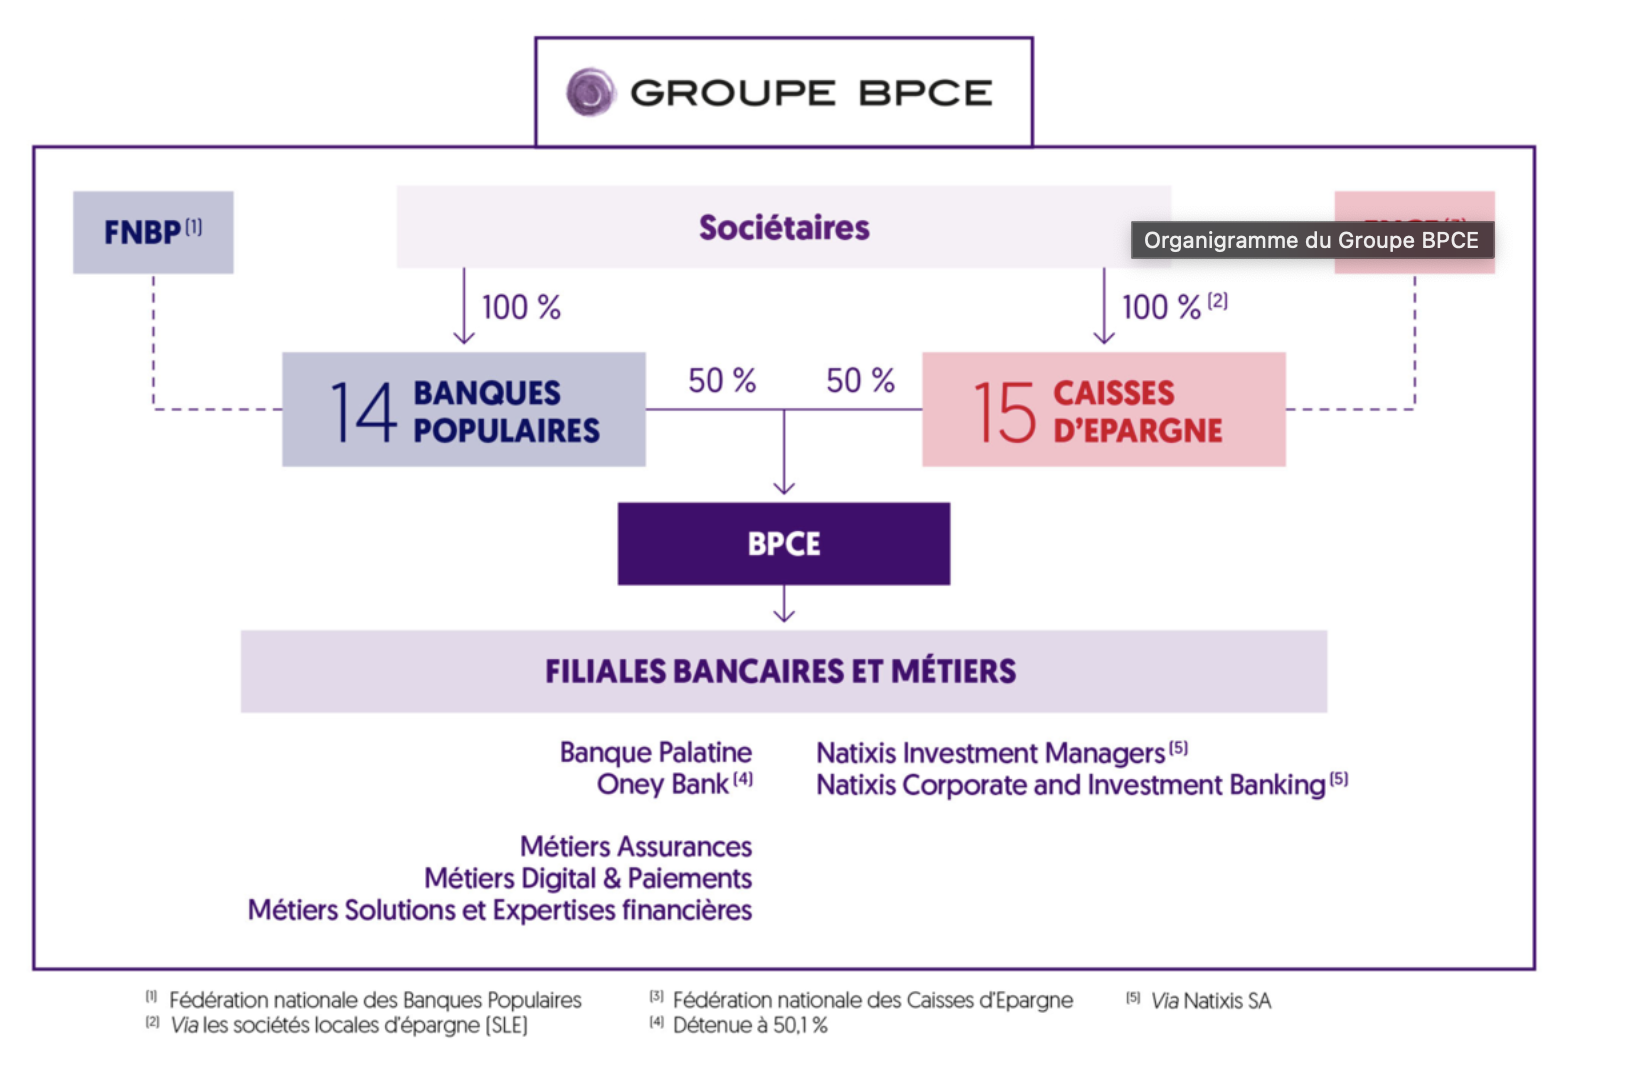
\includegraphics[width=\linewidth]{./img/intro/bpce_orga}
\end{figure}


\subsection*{Natixis Investment Managers}
%\addcontentsline{toc}{subsection}{Natixis Investment Managers} 
Natixis Investment Managers se fonde sur la force d’une approche indépendante en matière de gestion d’actifs. Chaque société de gestion affilée se concentre sur les styles et disciplines d'investissement pour lesquels elle dispose d'une expertise éprouvée. Il en résulte une sélection de plus de 200 stratégies d’investissement élaborées par des sociétés de gestion dont certaines figurent parmi les plus réputées au monde.

\begin{figure}[h!]
  \caption{Titre de la figure (source : \cite{ab94})}
  
\includegraphics[width=\linewidth]{./img/intro/nim_kpi}
\end{figure}


\begin{figure}[h!]
  \caption{Titre de la figure (source : \cite{m85})}
  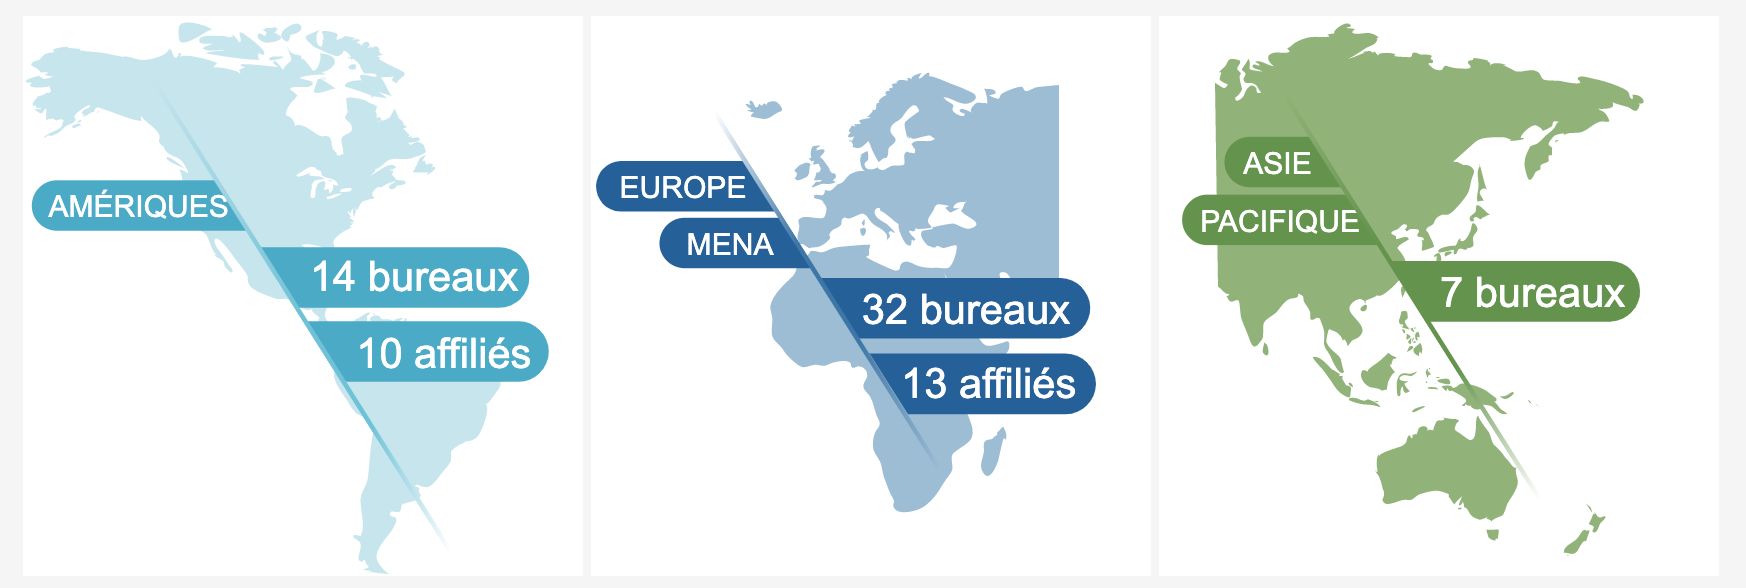
\includegraphics[width=\linewidth]{./img/intro/nim_loc}
\end{figure}



\subsection*{Seeyond}
%\addcontentsline{toc}{subsection}{Seeyond} 


\begin{figure}[h!]
  \caption{Titre de la figure (source : \cite{ah2006})}
  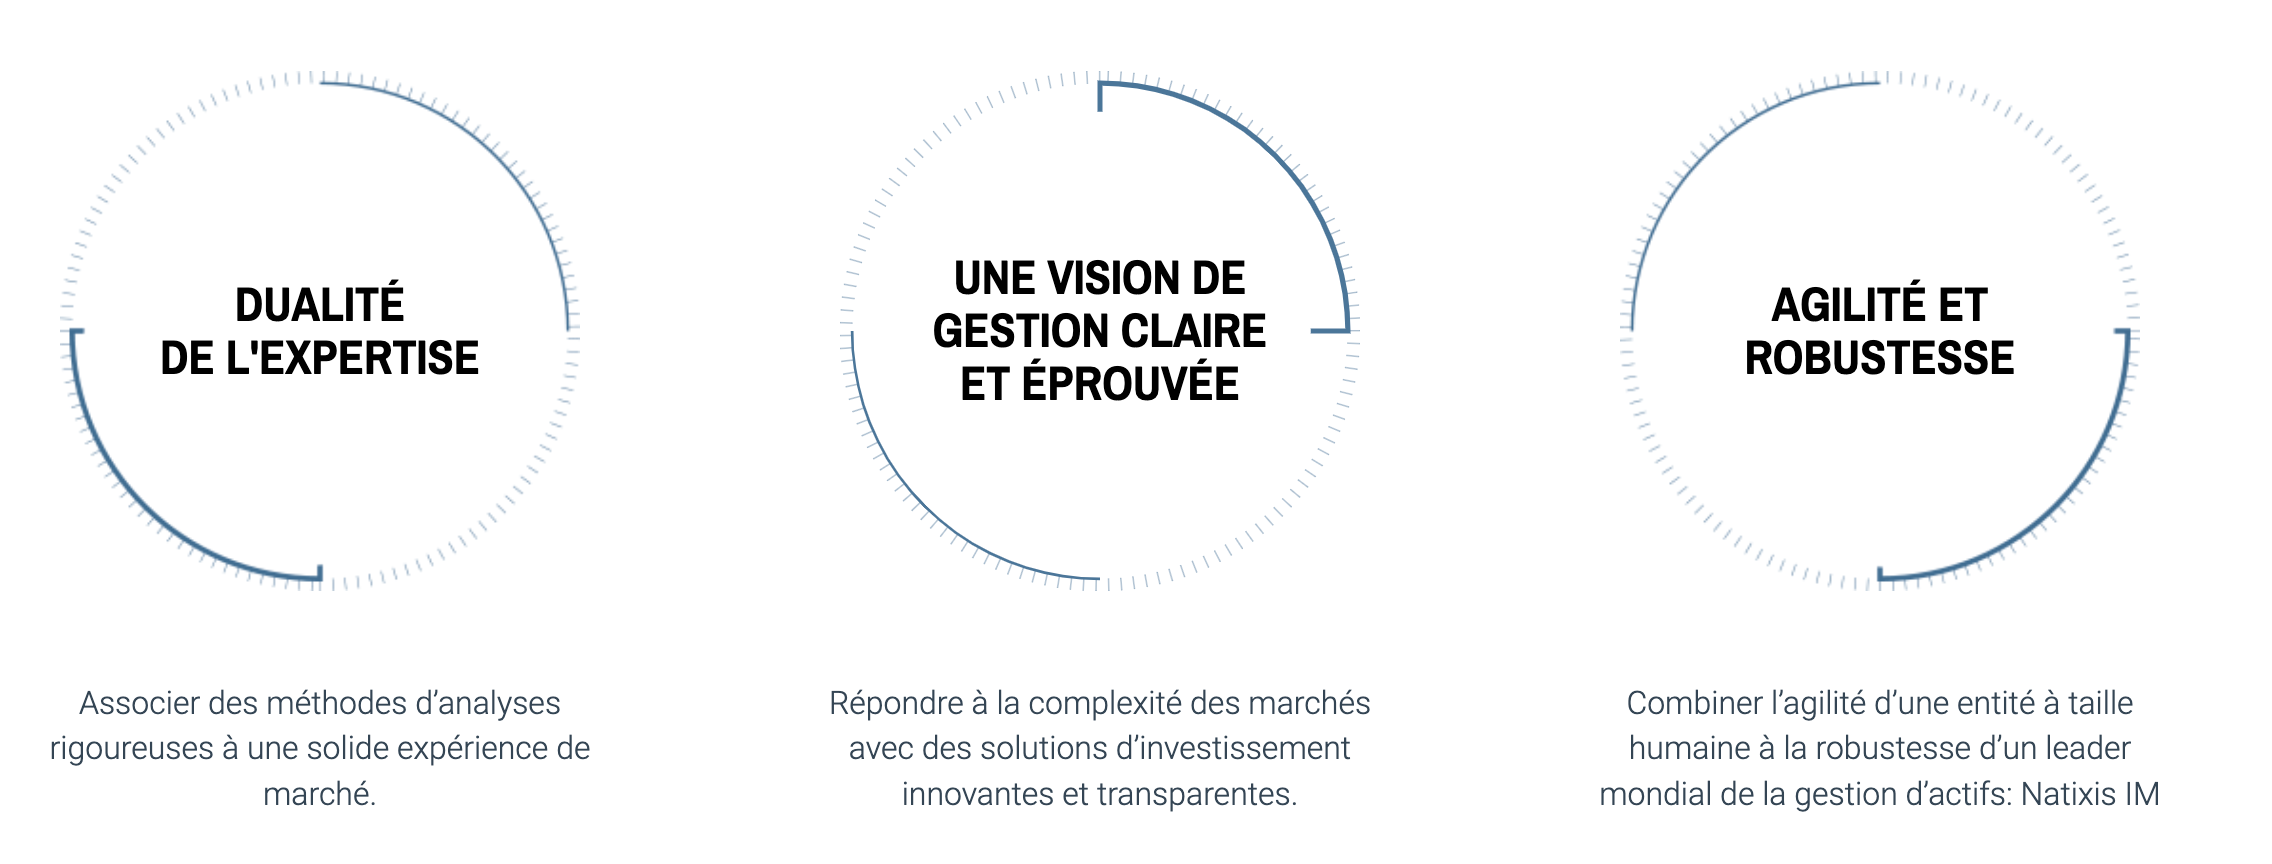
\includegraphics[width=\linewidth]{./img/intro/seeyond_objectifs}
\end{figure}

Seeyond est un spécialiste de la gestion quantitative active. A travers une approche intégrant une dimension humaine à la rigueur de processus d’investissement quantitatifs, les stratégies de gestion de Seeyond recherchent une rémunération optimale du risque, et ce sur trois expertises cœur : 
\begin{itemize}
\item Gestion Actions : Une expertise dont l’objectif est de transformer les primes de risque* actions et les anomalies de marché en source de performance.
\item Gestion Multi-asset : Une allocation active et flexible entre différentes classes d’actifs combinant convictions des gérants et indicateurs objectifs d’analyse de marché.
\item Gestion Volatilité \& Overlay : Des stratégies de gestion dédiées à la volatilité en tant que classe d’actifs.
\end{itemize}

Ces stratégies bénéficient de la longue expérience sur les marchés financiers et en analyse quantitative des professionnels de Seeyond.

\begin{figure}[h!]
  \caption{Titre de la figure (source : \cite{arrow48})}
  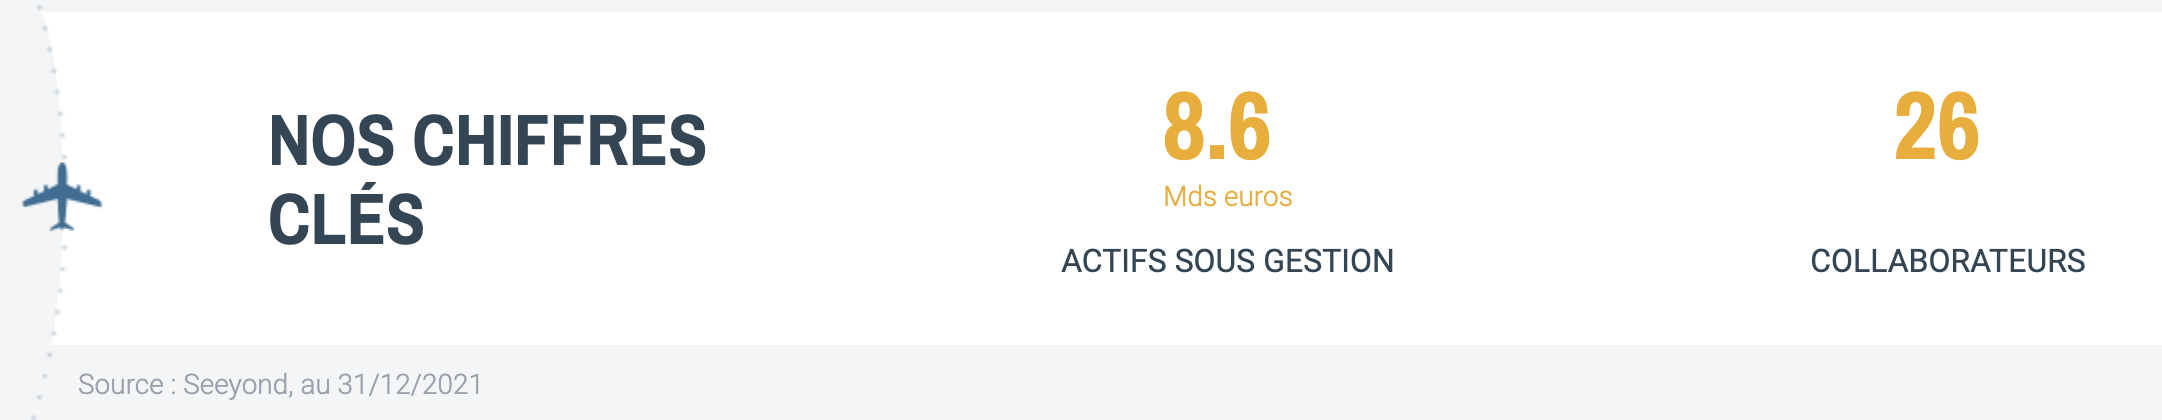
\includegraphics[width=\linewidth]{./img/intro/seeyond_kpi}
\end{figure}


En 2012, les équipes dédiées à la gestion quantitative* active du groupe Natixis Investment Managers, l’un des leaders mondiaux de la gestion d’actifs, ont été regroupées au sein d’une division de gestion dédiée avec une marque propre : Seeyond.
\\
En 2018, forte de son développement en tant que division de gestion, Seeyond est devenue une société indépendante et filiale à part entière du groupe Natixis IM.

\begin{figure}[h!]
  \caption{Titre de la figure (source : )}
  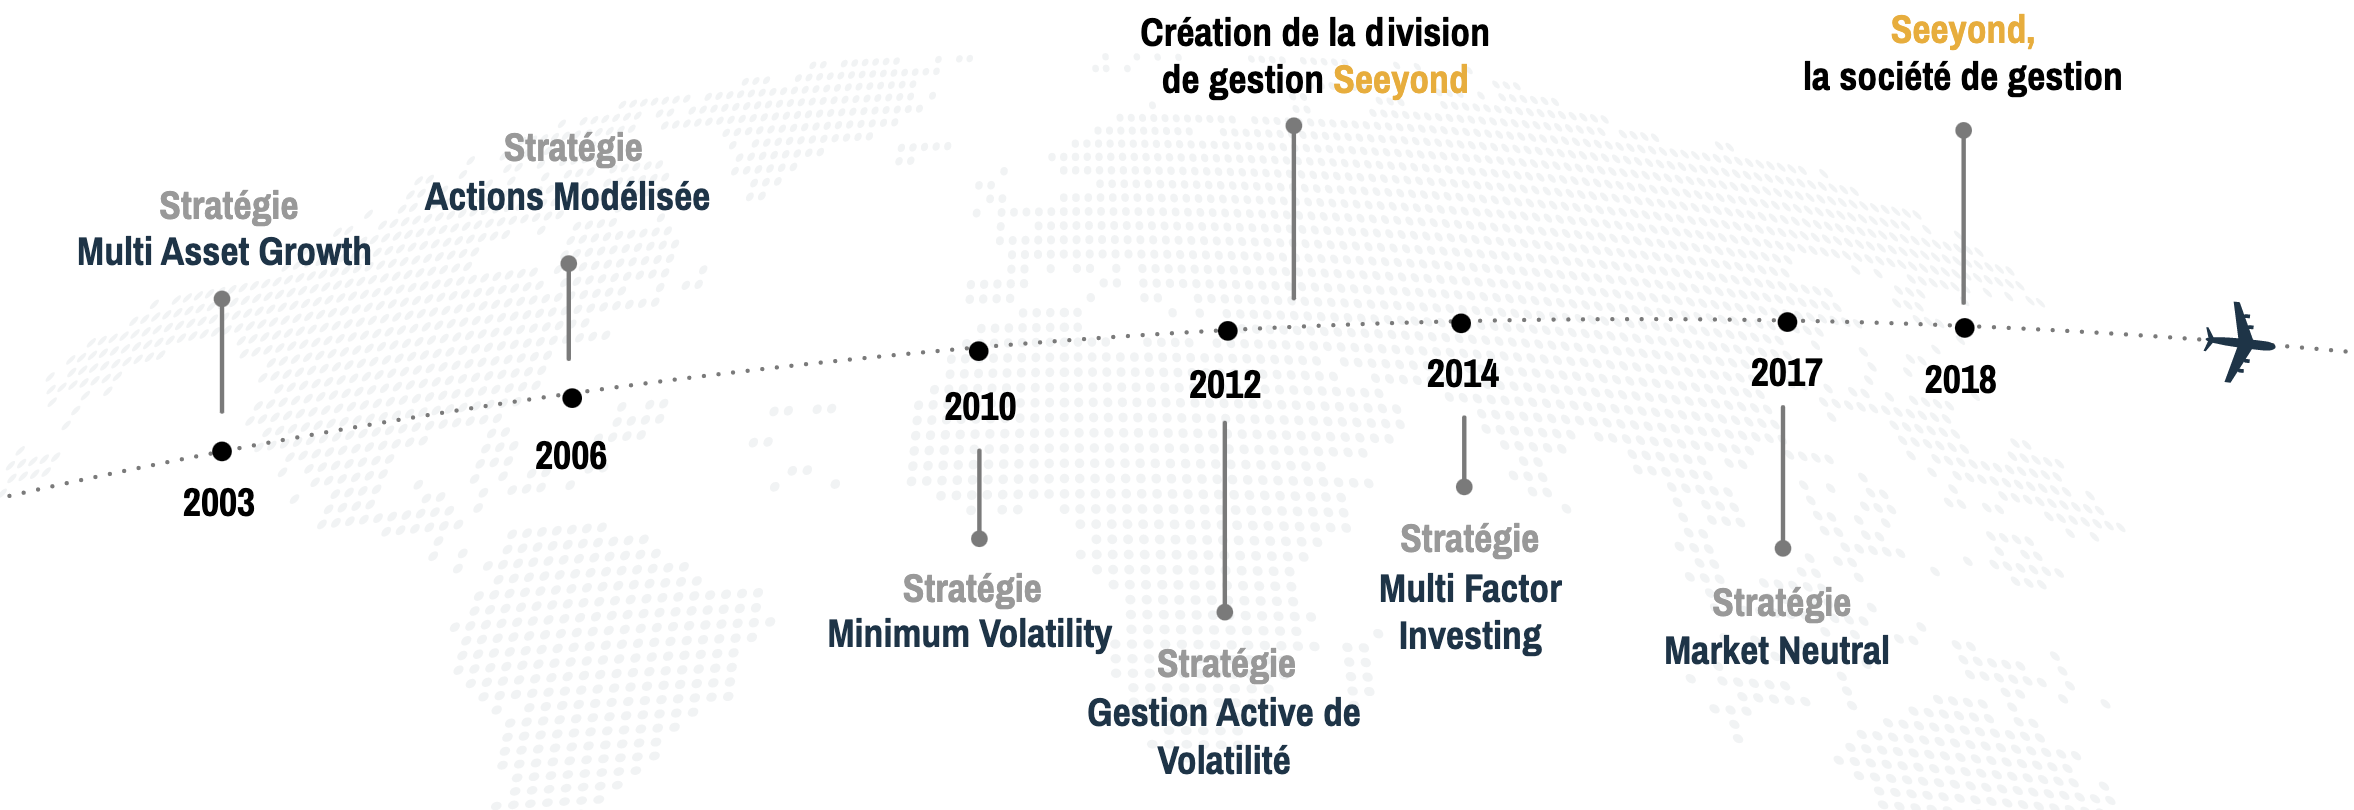
\includegraphics[width=\linewidth]{./img/intro/seeyond_hist}
\end{figure}



\newpage



\section*{Mon équipe}
%    \addcontentsline{toc}{section}{Mon équipe} 
Je fais parti de l'équipe RAD pour Rapid Application Development. La mission de cette équipe est de proposer un développement de proximité avec les différents services de Seeyond. Nous intervenons à la fois pour maintenir le système existant et pour développer de nouvelles fonctionnalités ou de nouveaux outils. Pour cela nous sommes en contact quotidiennement avec les membres de ces équipes afin de comprendre et répondre à leurs besoins.
\\
\\
Nous intervenons sur l'ensemble de la chaîne Front to Back, notamment avec la gestion, la recherche et la finance. Nous sommes amené à travailler sur des problématiques de gestion de portfeuille, de couvertures des risques, de suivie de transactions et bien d'autres.
\\
\\
Une de nos missions actuelle est de migrer les outils existant en VBA vers Python. L'intérêt de cette migration est de moderniser les outils en facilitant leurs développements futurs et en améliorant leur performance d'éxécution. De plus, nous profitons de cette migration pour regrouper l'ensemble des outils dans Enigma, une application web commune à toutes les équipes.

\newpage



\section*{Ma mission}
%\addcontentsline{toc}{section}{Ma mission} 
\subsection*{Mes réalisations}
\addcontentsline{toc}{subsection}{Mes réalisations} 
J'ai travaillé avec l'équipe RAD sur la maintenance des outils existants et sur de nouveaux développements. En particulier sur la migration d'outil VBA en python et sur leur intégration dans l'application Enigma.
\\
\\
J'ai par exemple travaillé sur un outil de calcul des commissions de sur-performance de certains fonds. En effet, Seeyond est un asset-manager qui se rémunère grâce aux frais récupérés des fonds sous-gestion. Des commissions de sur-performance s'appliquent sur certains portfeuilles Lorsqu'ils "battent" un indice qui sert de benchmark/comparatif. 
\\
Comme il peut s'agir de sommes importantes, ce calcul est réglementé. On le fait en interne et on doit le comparer à celui fait par un organisme externe. Il doit y avoir une trace/un historique de ces calculs.
\\
\\
J'ai aussi travaillé sur un outil permettant de générer divers graphiques sur les différents fonds gérés par Seeyond comme le drawdown sur une période donnée, la performance du fond par rapport à son benchmark, ... Cet outil est utilisé par les commerciaux afin de générer leurs présentations clients.

\subsection*{Problématique en lien avec l'équipe RAD}
%\addcontentsline{toc}{subsection}{Problématique en lien avec l'équipe RAD} 
La problématique de mon mémoire est d'utiliser l'algorithme UMAP (\textcolor{red}{le mot complet}) sur un jeu de données contenant diverses caractéristiques sur des actions depuis 1997.
\\
L'objectif est double, premièrement il faut essayer de repérer les caractéristiques des titres à faible volatilité qui sont susceptibles de voir leur volatilité augmenter à une horizon proche. Ensuite il faut améliorer la visualisation de ces données.
\\
\\
L'intérêt pour la gestion action est de pouvoir repérer les titres stables, pour assurer une certaine sécurité notamment en période de "crises".
\\
Il s'agit d'un problématique de recherche. ( Selon le résultat il n'y aura pas nécessairement la création d'un nouvel outil. ) 

\newpage


%%%%%%%%%%%%%%%%%%%%%%%%%%%%%%%%%%%%
% Partie Bibliographie
%%%%%%%%%%%%%%%%%%%%%%%%%%%%%%%%%%%%
%\newpage
%\onehalfspacing
%% Definition de l'en-tête
%\lhead[]{Recherche bibliographique}
% % Rajout Recherche bibliographique dans la TDM
%\addcontentsline{toc}{chapter}{\Large Recherche bibliographique}
%\chapter*{Recherche bibliographique}
%%%
%\newpage

%Partie recherche bibliographique avec les différentes parties et sections\


\section{ Section 1}
Lorem ipsum dolor sit amet, consectetur adipiscing elit. Sed non risus. Suspendisse lectus tortor, dignissim sit amet, adipiscing nec, ultricies sed, dolor. Cras elementum ultrices diam. Maecenas ligula massa, varius a, semper congue, euismod non, mi. Proin porttitor, orci nec nonummy molestie, enim est eleifend mi, non fermentum diam nisl sit amet erat. Duis semper. Duis arcu massa, scelerisque vitae, consequat in, pretium a, enim. Pellentesque congue. Ut in risus volutpat libero pharetra tempor. Cras vestibulum bibendum augue. Praesent egestas leo in pede. Praesent blandit odio eu enim. Pellentesque sed dui ut augue blandit sodales. Vestibulum ante ipsum primis in faucibus orci luctus et ultrices posuere cubilia Curae; Aliquam nibh. Mauris ac mauris sed pede pellentesque fermentum. Maecenas adipiscing ante non diam sodales hendrerit.

Ut velit mauris, egestas sed, gravida nec, ornare ut, mi. Aenean ut orci vel massa suscipit pulvinar. Nulla sollicitudin. Fusce varius, ligula non tempus aliquam, nunc turpis ullamcorper nibh, in tempus sapien eros vitae ligula. Pellentesque rhoncus nunc et augue. Integer id felis. Curabitur aliquet pellentesque diam. Integer quis metus vitae elit lobortis egestas. Lorem ipsum dolor sit amet, consectetuer adipiscing elit. Morbi vel erat non mauris convallis vehicula. Nulla et sapien. Integer tortor tellus, aliquam faucibus, convallis id, congue eu, quam. Mauris ullamcorper felis vitae erat. Proin feugiat, augue non elementum posuere, metus purus iaculis lectus, et tristique ligula justo vitae magna.
Aliquam convallis sollicitudin purus. Praesent aliquam, enim at fermentum mollis, ligula massa adipiscing nisl, ac euismod nibh nisl eu lectus. Fusce vulputate sem at sapien. Vivamus leo. Aliquam euismod libero eu enim. Nulla nec felis sed leo placerat imperdiet. Aenean suscipit nulla in justo. Suspendisse cursus rutrum augue. Nulla tincidunt tincidunt mi. Curabitur iaculis, lorem vel rhoncus faucibus, felis magna fermentum augue, et ultricies lacus lorem varius purus. Curabitur eu amet.

\section{Section 2}
Lorem ipsum dolor sit amet, consectetur adipiscing elit. Sed non risus. Suspendisse lectus tortor, dignissim sit amet, adipiscing nec, ultricies sed, dolor. Cras elementum ultrices diam. Maecenas ligula massa, varius a, semper congue, euismod non, mi. Proin porttitor, orci nec nonummy molestie, enim est eleifend mi, non fermentum diam nisl sit amet erat. Duis semper. Duis arcu massa, scelerisque vitae, consequat in, pretium a, enim. Pellentesque congue. Ut in risus volutpat libero pharetra tempor. Cras vestibulum bibendum augue. Praesent egestas leo in pede. Praesent blandit odio eu enim. Pellentesque sed dui ut augue blandit sodales. Vestibulum ante ipsum primis in faucibus orci luctus et ultrices posuere cubilia Curae; Aliquam nibh. Mauris ac mauris sed pede pellentesque fermentum. Maecenas adipiscing ante non diam sodales hendrerit.

Ut velit mauris, egestas sed, gravida nec, ornare ut, mi. Aenean ut orci vel massa suscipit pulvinar. Nulla sollicitudin. Fusce varius, ligula non tempus aliquam, nunc turpis ullamcorper nibh, in tempus sapien eros vitae ligula. Pellentesque rhoncus nunc et augue. Integer id felis. Curabitur aliquet pellentesque diam. Integer quis metus vitae elit lobortis egestas. Lorem ipsum dolor sit amet, consectetuer adipiscing elit. Morbi vel erat non mauris convallis vehicula. Nulla et sapien. Integer tortor tellus, aliquam faucibus, convallis id, congue eu, quam. Mauris ullamcorper felis vitae erat. Proin feugiat, augue non elementum posuere, metus purus iaculis lectus, et tristique ligula justo vitae magna.
Aliquam convallis sollicitudin purus. Praesent aliquam, enim at fermentum mollis, ligula massa adipiscing nisl, ac euismod nibh nisl eu lectus. Fusce vulputate sem at sapien. Vivamus leo. Aliquam euismod libero eu enim. Nulla nec felis sed leo placerat imperdiet. Aenean suscipit nulla in justo. Suspendisse cursus rutrum augue. Nulla tincidunt tincidunt mi. Curabitur iaculis, lorem vel rhoncus faucibus, felis magna fermentum augue, et ultricies lacus lorem varius purus. Curabitur eu amet.

%\newpage

%%%%%%%%%%%%%%%%%%%%%%%%%%%%%%%%%%%%
% Chapitre 1
%%%%%%%%%%%%%%%%%%%%%%%%%%%%%%%%%%%%

% Definition de l'en-tête
\lhead[]{Chapitre 1 : Présentation de la problématique}
\newpage
   % Inclut fichier tex du Chapitre 1
   \chapter{Présentation de la problématique}

\section{Aspect métier}

\subsection{Pourquoi c'est important ce sujet ?}
Ce sujet est important pour la gestion action. En effet, comme vu précedemment Seeyond propose trois types de produits: les fonds Actions, les fonds Multi-asset et les fond Volatilité et Overlay.
\\
Les fonds Actions sont exclusivement composés de titres d'entreprise ce qui rend compliqué leur gestion en période de crise. En effet, Seeyond étant un asset-manager, un certain de niveau de performance est attendu de la part des clients. C'est pourquoi en période de crise, les gérants de portefeuille s'interessent aux titres à faible volatilité, dit Low-vol.
\\
\\
Nous disposons de multiples données sur des titres d'entreprises. Certaines comme le prix de l'action, la market cap (capitalisation) et bien d'autres sont récupérés via des sources externes comme Bloomberg; tandis que d'autre sont directement calulées par l'equipe quantitative (recherche) comme la volatilité, le momementum, ...
\\
L'utilisation d'un algorithme à réduction de dimension pourrait donc être pertinente dans notre cas. C'est pourquoi nous aimerions voir si UMAP peut nous aider à identifier des caractéristiques communes aux titres Low-vol. Voir même en allant plus loin à identifier les caractéristiques des titres Low-vol qui vont changer de régime (ne seront plus Low-vol).
\\
Il est évident que pouvoir anticiper l'identification des titres à faible volatilité, et possiblement leur changement de régime, serait un avantage non négligeable dans la gestion de portefeuille actions. Il serait ainsi possible d'optimiser les performances en période de crise en se positionnant plus efficacement dans les valeurs refuges (low-vol).

\subsection{Définition de la low-vol et fréquence}
Les titres low-vol sont des titres à faible volatilité. C'est à dire que leur prix évolue peu (en valeur).


\section{Aspect technique}

\subsection{Pourquoi c'est riche comme sujet ?}
C'est un sujet vaste, nous allons aborder de nombreuses notions comme le fléau de la dimension lorque l'on travaille en grande dimension et l'intérêt des algorithmes de réduction de dimension pour palier à ce problème.
\\
Nous allons traiter de UMAP, des intuitions derrières cet algorithme et des avantages/différences comparées aux algorithmes existants.


\section{Données/cadre de travail}

\subsection{Avec quoi/qui/comment tu bosses ?}
J'ai travaillé conjointement avec l'équipe Recherche, la Gestion Action de qui vient la demande et l'équipe RAD sur ce projet. J'étais le principal interlocuteur de l'équipe RAD sur ce sujet même si l'ensemble de l'équipe restait informé du sujet. 
\\
L'équipe Recherche avait le lead sur ce projet. Je travaillai puis validais l'avancée avec la recherche qui m'indiquait la suite du travail et m'aidait dans mes interprétations.
\\
J'ai travaillé sur ce projet en autonomie et sur d'autres projet en parallèle durant ma mission. 

\subsection{Exploitation transformations des données}
Le jeu de données a été fourni par l'équipe Recherche. Il comprend diverses informations sur des titres d'entreprises (environ 1800 - de diverses régions et divers secteurs) de 1997 à 2017. Les informations sur ces titres sont récupérés de sources externes comme Bloomberg ou ont eté calculées par l'équipe Recherche.
   % Termine le Chapitre 1
   \newpage
   
%Bibliographie du Chapitre 1
 %  \bibliography{biblio}
   % Termine la biblio du Chapitre 1
   %\newpage









%%%%%%%%%%%%%%%%%%%%%%%%%%%%%%%%%%%%
% Chapitre 2
%%%%%%%%%%%%%%%%%%%%%%%%%%%%%%%%%%%%

% Definition de l'en-tête
\lhead[]{Chapitre 2 : Notions mathématiques}
\newpage
   % Inclut fichier tex du Chapitre 2
   \chapter{Notions mathématiques}

Nous allons traiter dans cette section de notions mathématiques qui seront abordées dans la suite de ce mémoire. Ce sont des notions importantes pour notre bonne compréhension du sujet et de ses enjeux.

\section{Métriques et Espaces métriques}

\subsection*{Métriques}
Une métrique est une mesure de distance, c'est une fonction qui retourne la distance entre deux points. Dans le plan cartésien, on sait que la distance entre deux points $(x_1, y_1)$ et $(x_2, y_2)$ est donnée par la formule de distance : \\
$$ \sqrt{(x_2 - x_1)^2 - (y_2 -y_1)^2} $$

%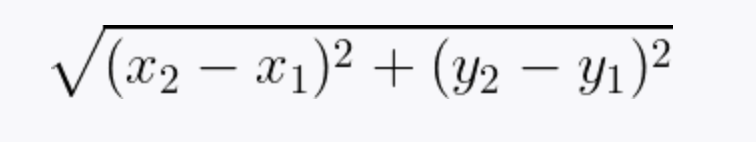
\includegraphics[width=100pt]{./img/notions_math/metric/eq_cartesienne}


C'est généralement la façon dont nous pensons à la distance. Mais dans de nombreuses situations réelles, nous ne pouvons pas penser à nos points de données d'une manière qui aurait le sens géométrique.
\\
Par exemple, imaginons que nous avons une courbes de prix des actions de deux sociétés différentes. Disons que $f(t)$ est une fonction représentant le prix d'une action au temps $t$ et $g(t)$ représente le prix d'une autre action au temps $t$. Quelle est la distance entre les fonctions $f$ et $g$ ? 
\\
Pour répondre à cette question, nous ne pouvons pas utiliser la formule de distance vu précedemment. Nous avons besoin d'une définition plus générale. 
\\
\\
Supposons que $X$ soit un ensemble quelconque. Nous définissons une métrique sur $X$ comme une fonction de distance $d$ qui satisfait les axiomes suivants :
\begin{enumerate}
        \item $d(x, x)=0$ pour tout $x \in X$
        \item $d(x, y)=d(y, x)$ pour tout $x,y \in X$
        \item $d(x, y) \geqslant 0$ pour tout $x, y, z \in X$
        \item $d(x, y) \leqslant d(x, z) + d(z, y)$ pour tout $x, y, z \in X$
\end{enumerate}

Le premier axiome signifie que chaque élément de x est à une distance 0 de lui-même. Le deuxième axiome signifie que la distance de x à y est la même que la distance de y à x. Puisque la distance négative n'a pas de sens, le troisième axiome garantit que deux points n'ont pas de distance négative l'un par rapport à l'autre. Le dernier axiome, et le plus important, est connu sous le nom d'inégalité triangulaire. La règle du triangle est l'une des inégalités les plus importantes des mathématiques, malgré sa simplicité. Elle stipule essentiellement que la somme des deux côtés d'un triangle est supérieure à l'un de ses côtés.
\\
\\
Nous allons examiner quelques métriques intéressantes pour mieux comprendre l'intérêt d'utiliser des métriques différentes. Elles vérifient évidement toutes les précedents axiomes.


\textbf{Métrique discrète}
\\
Pour tout ensemble $X$, la métrique discrète est définie comme suit :

%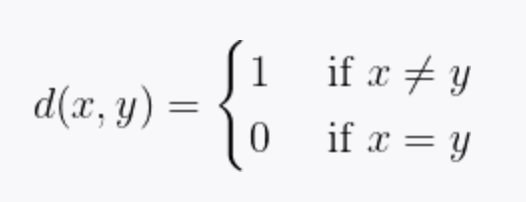
\includegraphics[width=100pt]{./img/notions_math/metric/metric_discret}
\[ d(x,y) =
  \begin{cases}
    1       & \quad \text{si } x \ne y \\
    0       & \quad \text{si } x = y 
  \end{cases}
\]



\textbf{Valeur absolue}
\\
Dans $\mathbb{R}$, l'ensemble de tous les nombres réels, la fonction : 

%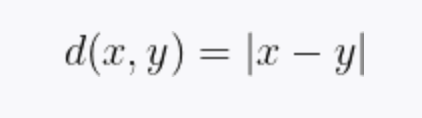
\includegraphics[width=100pt]{./img/notions_math/metric/val_abs}
$$ d(x,y) = \lvert x - y \rvert$$

\textbf{Fonction continue}
\\
Soit $C[0, 1]$ l'espace des fonctions continues avec le domaine [$0, 1]$. Il existe plusieurs métriques que l'on peut placer sur cet espace :

%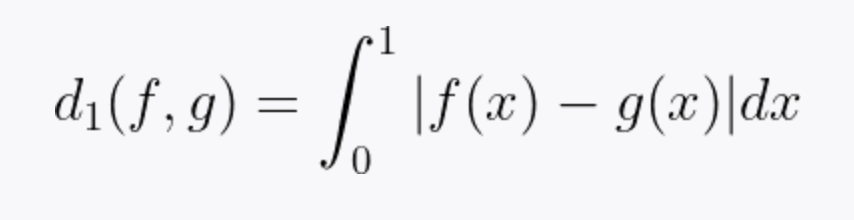
\includegraphics[width=100pt]{./img/notions_math/metric/eq_fcn_con_1_1}
$$ d_1(f,g) = \int_0^1  \lvert f(x) - g(x) \rvert dx$$


Cela définit l'aire totale entre deux fonctions $f$ et $g$ : 


\begin{figure}[h!]
  \caption{Titre de la figure (source : \cite{arrow48})}
  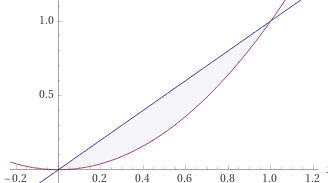
\includegraphics[width=200pt]{./img/notions_math/metric/courbe_metric_fcn}
\end{figure}

En général, si f et g sont deux fonctions dans C[a, b], alors on définit pour tout p >= 1 :

%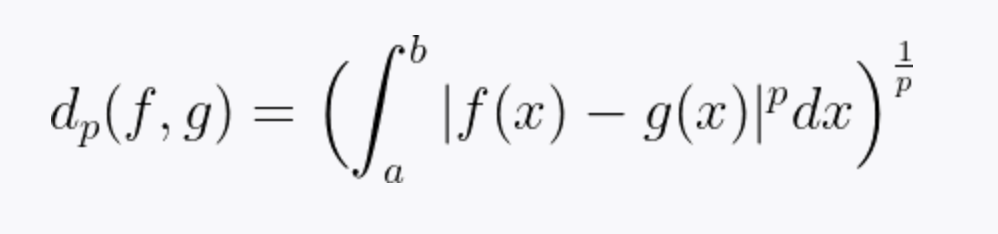
\includegraphics[width=100pt]{./img/notions_math/metric/eq_fcn_con_1_2}
$$ d_p(f,g) = (\int_a^b  \lvert f(x) - g(x) \rvert ^p dx)^{1/p}$$

\textit{Une autre métrique continue}
Soit $C[a, b]$ l'espace des fonctions continues avec le domaine $[a, b]$. Nous pouvons définir la métrique suivante comme êtant la distance maximale entre $f$ et $g$ dans l'intervalle $[a, b] $: 

%
\includegraphics[width=100pt]{./img/notions_math/metric/eq_fcn_con_2}
$$ d_\infty(f,g) = max \left\{  \lvert f(x) - g(x) \rvert : x \in [a,b] \right\}
$$

    
\section*{Espaces Métrique}
Maintenant que nous avons une idée de ce qu'est une métrique, nous pouvons définir les espaces métriques. Un espace métrique est une paire (X, d) où X est un ensemble, et d est une métrique définie sur des points de l'ensemble X. Nous venons de voir plusieurs exemples d'espaces métriques ci-dessus. Nous allons maintenant examiner certaines propriétés importantes des espaces métriques.
\\
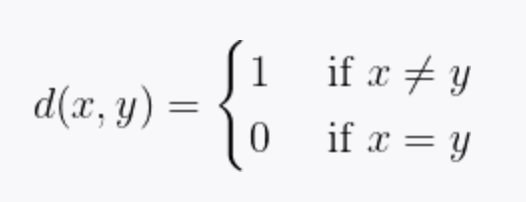
\includegraphics[width=100pt]{./img/notions_math/metric/metric_discret.png}
\\
Soit (X, d) un espace métrique, et soit $x_0$ un élément quelconque de X. Pour un certain $r > 0$ fixé, définissez la boule ouverte de rayon r centrée sur $x_0$ par l'ensemble ci-dessous (aussi écrit $B(x_0 ; r)$): 
\\
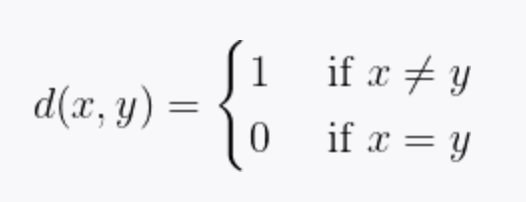
\includegraphics[width=100pt]{./img/notions_math/metric/metric_discret.png}



\section*{Cosine Distance}
Nous allons nous intésser à la distance cosinus (ainsi  qu'à la similarité cosinus). En effet, comme nous allons le  voir plus tard, cette mesure peut être intéressantes dans notre utilisation de UMAP. En effet, nous verrons que le choix de la métrique peut avoir une influence intéressante sur l'algorithme et nous allons essayer de comprendre pourquoi cette métrique peut être particulièrement adapté à notre problème (ou pas).
\\
\\
Pour commencer nous allons définir la similarité en cosinus. Il s'agit d'une métrique qui mesure le cosinus de l'angle entre deux vecteurs projetés dans un espace multidimensionnel.


Plus l'angle entre les deux vecteurs est petit, plus ils sont similaires l'un à l'autre; Donc plus la similarité cosinus se rapproche de 1, plus l'angle entre les deux vecteurs A et B est faible. Dans ce cas, A et B sont plus similaires l'un à l'autre.
\\
Supposons maintenant que l'angle entre les deux vecteurs soit de 90 degrés, la similitude en cosinus aura une valeur de 0. Cela signifie que les deux vecteurs sont perpendiculaires l'un à l'autre, ce qui signifie qu'il n'y a aucune corrélation entre eux.
\\
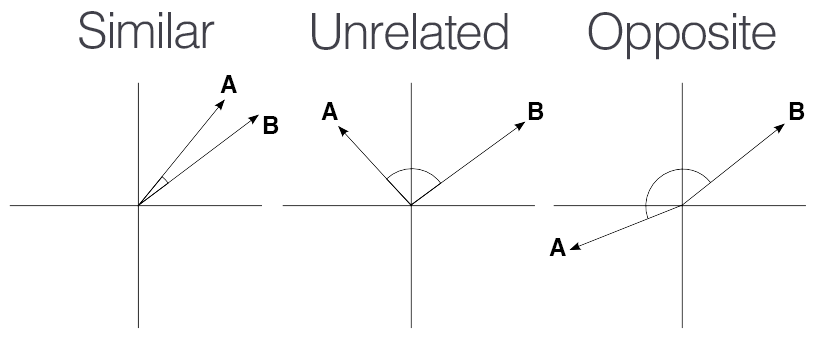
\includegraphics[width=200pt]{./img/notions_math/metric/img_metric_cos.png}


La similarité en cosinus est décrite mathématiquement comme la division entre le produit scalaire des vecteurs et le produit des normes euclidiennes ou de la magnitude de chaque vecteur :


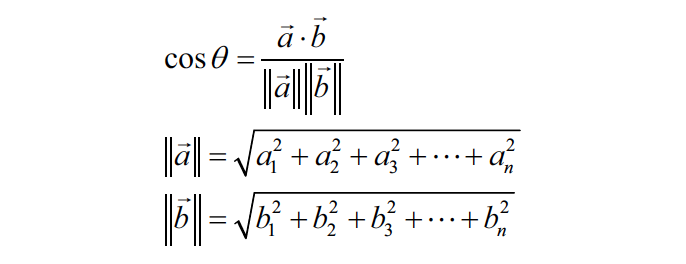
\includegraphics[width=200pt]{./img/notions_math/metric/eq_metric_cos.png}
\\
Où, a et b sont des vecteurs dans un espace multidimensionnel.


Puisque la valeur $\cos(\theta)$ est comprise dans l'intervalle [-1,1] :
\begin{itemize}
    \item La valeur -1 indiquera des vecteurs fortement opposés, c'est-à-dire aucune similarité.
    \item 0 indique des vecteurs indépendants (ou orthogonaux).
    \item 1 indique une forte similarité entre les vecteurs.
\end{itemize}
La distance cosinus est définit comme :
\begin{eqnarray}
    Cosine Distance = 1 — Cosine Similarity
\end{eqnarray}
L'intuition derrière cela est que si 2 vecteurs sont parfaitement identiques alors la similarité est de 1 (angle=0 donc $\cos(\theta)$=1) et donc, la distance est de 0 (1-1=0).
\\
\\
La distance du cosinus est utilisée dans de nombreux domaines, par exemple :
\begin{enumerate}
    \item Cette métrique est utilisée dans les processus d'exploration de données, de recherche d'informations et de mise en correspondance de textes.
    \item Elle est aussi utilisé dans les moteurs de recommandation pour recommander des produits/films/spectacles/livres similaires.
    \item Dans le domaine de la recherche d'informations, l'utilisation de TF-IDF pondéré et de la similarité en cosinus est une technique très courante pour retrouver rapidement les documents similaires à une requête de recherche.
\end{enumerate}



\newpage







\section{Fléau de la dimension}
De nombreux jeux de données impliquent des milliers, voire des millions de caractéristiques pour chaque observation. Toutes ces caractéristiques peuvent rendre l'apprentissage extrêmement lent, mais elles peuvent aussi rendre beaucoup plus difficile la recherche d'une bonne solution. Ce problème est souvent appelé fléau de la dimension.
\\
Si nous avons plus de caractéristiques que d'observations, nous courons le risque de surajuster massivement (overfitting) notre modèle. Cela ce traduit généralement par des performances hors échantillon épouvantables.
\\
Lorsque nous avons trop de caractéristiques, les observations deviennent plus difficiles à regrouper. Trop de dimensions font que chaque observation du jeu de données semble équidistante de toutes les autres. Et comme le clustering utilise une mesure de distance telle que la distance euclidienne pour quantifier la similarité entre les observations, c'est un gros problème. Si les distances sont toutes approximativement égales, alors toutes les observations semblent également similaires (ainsi qu'également différentes), et aucun cluster significatif ne peut être formé.
\\
\\
Le fait d'avoir trop de caractéristiques peut perturber certains algorithmes de machine learning tels que les algorithmes de clustering. La réduction de la dimensionnalité peut aider à améliorer les performances de ceux-ci.
\\
Dans le monde réel les données souvent désordonnées avec du bruit et des relations compliquées. La réduction de la dimensionnalité représente un compromis entre un modèle potentiellement plus robuste et une interprétabilité moindre.
\\
\\
\\
\\
Georg Cantor est un mathématicien allemand du 19e siècle qui est particulièrement connu pour son travail sur la théorie des ensembles et plus spécifiquement sur ses résultats concernant l’infini. L’ensemble des nombres entier est infini par construction, mais l’ensemble des nombres entier relatif également. Et intuitivement, nous nous disons que ces infini ne sont pas vraiment les mêmes, puisqu’il semblerait que Z soit plus grand que N ! Georg Cantor montre que ces deux infini sont en fait les mêmes : il y a autant de nombres dans Z que dans N. Plus fort encore, il démontre la puissance de l’infini qui nous donne un résultat encore plus contre intuitif : il y a autant de nombre dans l’interval $[0, 1]$ que dans R tout entier ! Alors qu’il venait de le démontrer, il a envoyé une lettre à son ami mathématicien Dedekind :
\begin{quotation}
    Tant que vous ne m’aurez pas approuvé, je ne puis que dire : je le vois mais je ne le crois pas.
    \\
    Georg Cantor (1877)
\end{quotation}
Il a prouvé quelque chose que l’ensemble de la communauté pensait intuitivement fausse, et lui-même n’y croyait pas. Nous sommes toujours mis en difficulté quand il s’agit de traiter avec l’infini, ou des grandes quantités. Cette remarque nous amène donc à nous questionner sur l’impact d’un grand nombre d’informations quand nous entraînons un modèle de Machine Learning.
\\
\\
Le fléau de la dimension est un phénomène connu en statistique et en Machine Learning. Ce terme rassemble tout un ensemble de phénomène qui se produisent en très grande dimension, mais pas dans une dimension plus petite. Nous proposons dans cette annexe d’illustrer quelque-uns des phénomènes étranges de la grande dimension et ses impacts en Machine Learning.
\begin{quotation}
    The curse of dimensionality is taught in every Machine Learning programs, and refers to \textit{various phenomea that arise when analyzing and organizing data in high-dimensional spaces that do not occur in low-dimensional settings}\footnote{Definition from Wikipedia}. Living in a three dimensional world, it is known to be hard for human to apprehend infinity\footnote{e.g. the Cantor's work in mathematics with infinite set in set theory.}. Not fully understanding what the curse of dimensionality was as a student, I decided to look for strange behavior in high-dimension, hoping that it would shed light on the dimension curse.
\end{quotation}
\textbf{Volume d’une hypersphère}
Pour essayer de sentir les problèmes de la très grande dimension, on s’intéresse au volume d’une hypersphère.
\\
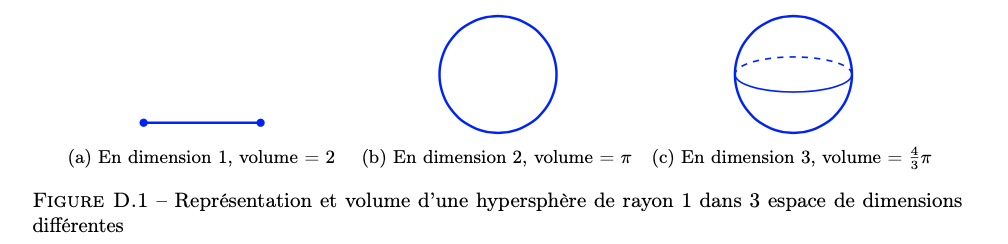
\includegraphics[width=\linewidth]{./img/notions_math/hypersphere_1}
\\
Avec la figure ci-dessus nous avons l’intuition que le volume augmente avec la dimension. Donc pour une hypersphère de très grande dimension, on devrait avoir un très grand volume.
\\
Nous avons tracé et mesuré le volume pour la distance euclidienne classique, mais nous pouvons aussi utiliser d’autre distance (autre norme) comme montré dans la figure ci-dessous.
\\
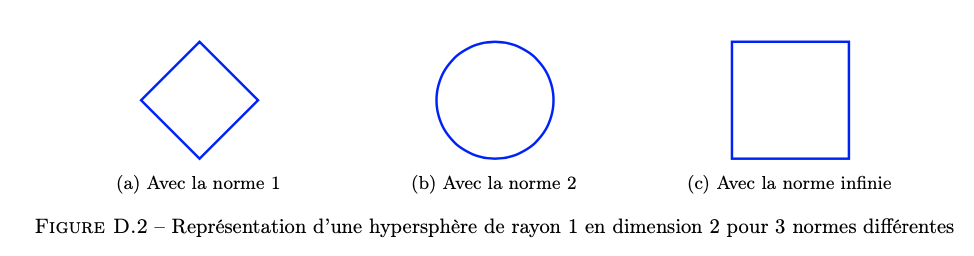
\includegraphics[width=\linewidth]{./img/notions_math/hypersphere_2}
\\
Formalisons le problème et généralisons-le pour calculer le volume d’une hypersphère en n’importe quelle dimension et pour n’importe quelle norme. Soit $n \in \mathbb{N}^*$ la dimension de l’espace, on appelle boule ou hypersphère l’objet défini par :

\begin{eqnarray*} 
    B_n^p(R) &=& \{ (x_1, \ldots, x_n) \in \mathbb{R}^n, \sum_{i=1}^n x_i^p \leqslant R^p\} \\
    &=& \{ u \in \mathbb{R}^n, \|u\|_p^p \leqslant R^p\}
\end{eqnarray*}

Nous savons que $\|u\|_p$ est la norme $p$ définit comme $\|u\|_p^p=\sum_{i=1}^n x_i^p$. $B_n^p(R)$ est la boule de dimension $n$ avec une norme $p$ de rayon $R$. On définit $V_n^p(R)$ le volume de la boule $B_n^p(R)$ \textit{i.e.} la measure de $B_n^p(R)$ pour la mesure de Lesbegue dans $\mathbb{R}^n$. Formellement :
\\
\begin{equation*} V_n^p(R) = \int_{B_n^p(R)} \bigotimes_{i=1}^n\mathrm{d}x_i \end{equation*}
\\
On définit la focntion:
\\
\begin{equation*}
\begin{array}{ccccc}
\phi & : & B_n^p(1) & \to & B_n^p(R) \\
& & (x_1, \ldots, x_n) & \mapsto & (Rx_1, \ldots, Rx_n) \\
\end{array}
\end{equation*}
Nous avons cela pour $u\in B_n^p(1)$, ensuite $\|u\|_p^p \leqslant 1 \Longleftrightarrow \|Ru\|_p^p \leqslant R^p$ donc $\phi(u) \in B_n^p(R)$, sous l'hypothèse $R>0$. 
Par équivalence, nous avons $\phi(B_n^p(1)) = \phi(B_n^p(R)$. $\phi$ est alors une correspondance biunivoque, alors par changement de variable on a : $V_n^p(R) = R^nV_n^p(1)$.
\\
Donc par Fubini :
\begin{eqnarray*}
V_n^p(1) &=& \int_{-1}^1 V_{n-1}^p\left(\sqrt[p]{1 - |x|^p}\right)\mathrm{d}x\\
&=& V_{n-1}^p(1) \int_{-1}^1 \left(1-|x|^p\right)^{\frac{n-1}{p}} \mathrm{d}x\\
&=& 2V_{n-1}^p(1) \int_0^1 \left(1-|x|^p\right)^{\frac{n-1}{p}} \mathrm{d}x\\
&=& \frac{2}{p} V_{n-1}^p(1) \int_0^1 y^{\frac{1}{p}-1}(1-y)^{\frac{n-1}{p}}\mathrm{d}y\\
\end{eqnarray*}
On rappelle la définition de la fonction Bêta définie pour $x, y \in \mathbb{R}_+^*$ :
\begin{equation*} B(x, y) = \int_0^1 t^{x-1}(1-t)^{y-1}\mathrm{d}t \end{equation*}
Nous connaissons aussi l'identité :
\begin{equation*} B(x, y) = \frac{\Gamma(x) \Gamma(y)}{\Gamma(x+y)} \end{equation*}

\textbf{La fonction Bêta}
\\
\\
Nous prouvons ici l'identité que nous avons utilisée pour trouver l'expression exacte du volume d'une boule en dimension $n$ en utilisant la distance $p$-normale. La fonction bêta est définie comme dit précédemment :
\\
\begin{equation*} B(x, y) = \int_0^1 t^{x-1}(1-t)^{y-1}\mathrm{d}t \end{equation*}
Pour $x,y > 0$. Et nous utilisons l'identité suivante :

%\lemme{Let $x, y \in \mathbb{R}_+^*$, we have :

%\begin{equation*} B(x, y) = \frac{\Gamma(x) \Gamma(y)}{\Gamma(x+y)} \end{equation*}
%}
\begin{proof}
Nous avons :

\begin{eqnarray*}
\Gamma(x)\Gamma(y) &=& \int_0^{+\infty} e^{-a}a^{x-1}\mathrm{d}a \times  \int_0^{+\infty} e^{-b}b^{x-1}\mathrm{d}b\\
&=& \int_{a=0}^{+\infty} \int_{b=0}^{+\infty} e^{-(a+b)}a^{x-1}b^{y-1}\mathrm{d}b\mathrm{d}a
\end{eqnarray*}

Nous effectuons le changement de variables : $u=a+b$ et $\displaystyle v=\frac{a}{a+b}$, qui est équivalent à $a=uv$ et $b=u(1-v)$. Nous avons maintenant :
\\
\begin{eqnarray*}
\Gamma(x)\Gamma(y) &=& \int_0^1\int_0^{+\infty} (uv)^{x-1}\left[u(1-v)\right]^{y-1}e^{-[uv+u(1-v)]}|-u|\mathrm{d}u\mathrm{d}v\\
&=& \int_0^1\int_0^{+\infty}u^{x+y-1}v^{x-1}(1-v)^{y-1}e^{-u}\mathrm{d}u\mathrm{d}v\\
&=& \int_0^1 v^{x-1}(1-v)^{y-1}\mathrm{d}v \times \int_0^{+\infty}u^{x+y-1}e^{-u}\mathrm{d}u\\
&=& B(x, y)\Gamma(x+y)
\end{eqnarray*}
\end{proof}



Nous pouvons alors écrire :
\begin{eqnarray*}
V_n^p(1) &=& \frac{2}{p} V_{n-1}^p(1) \frac{\Gamma\left(\frac{1}{p}\right)\Gamma\left(\frac{n-1}{p}+1\right)}{\Gamma\left(\frac{n}{p} + 1\right)}
\\
&=& V_{n-1}^p(1) \left[\frac{2}{p} \frac{\Gamma\left(\frac{1}{p}\right)\Gamma\left(\frac{n-1}{p}+1\right)}{\Gamma\left(\frac{n}{p} + 1\right)} \right]
\\
&=& V_1^p(1)2^{n-1}\Gamma\left(\frac{1}{p}+1\right)^{n-1} \frac{\Gamma\left(\frac{1}{p}+1\right)}{\Gamma\left(\frac{n}{p}+1\right)}
\\
&=& V_1^p(1)2^{n-1}\frac{\Gamma\left(\frac{1}{p}+1\right)^n}{\Gamma\left(\frac{n}{p}+1\right)}
\\
\end{eqnarray*}
Depuis $V_1^p(1) = 2$, nous obtenons la formule finale : 
\begin{equation*} \forall n\geqslant 2, \forall p\geqslant 1,  \; \; \;  V_n^p(1) = \frac{\left(2\Gamma\left(\frac{1}{p}+1\right)\right)^n}{\Gamma\left(\frac{n}{p}+1\right)} \end{equation*}
Donc avec un rayon, nous avons :
\\
\begin{equation} \forall R>0, \forall n\geqslant 2, \forall p\geqslant 1, \; \; \; V_n^p(R) = \frac{\left(2R\Gamma\left(\frac{1}{p}+1\right)\right)^n}{\Gamma\left(\frac{n}{p}+1\right)} \end{equation}
Nous aimerions savoir comment il se comporte en haute dimension, \textit{i.e.} pour $n$ assez grand. Nous savons que $\Gamma(n+1) = n!$ pour tout $n\in\mathbb{N}$. Donc nous utilisons cela pour l'équivalence :
\\
\begin{equation} 
V_n^p(R) \sim \sqrt{\frac{p}{2\pi n}} \left[2R\Gamma\left(\frac{1}{p}+1\right) \left(\frac{pe}{n}\right)^{\frac{1}{p}}\right]^n 
\end{equation}




Ce que ce résultat exhibe, c’est que le volume d’une hypersphère en grande dimension tend exponentiellement vite vers 0, c’est complètement contre intuitif ! Traçons des courbes de cette fonction :
\\
\\
Tout d'abord, nous voyons le premier fait surprenant : le volume qui augmente avec n converge vers 0 pour toute dimension métrique p ou tout rayon R. Avec notre intuition dans un monde tridimensionnel, nous nous attendions à ce que le volume augmente à l'infini. On peut regarder différentes courbes :
\\
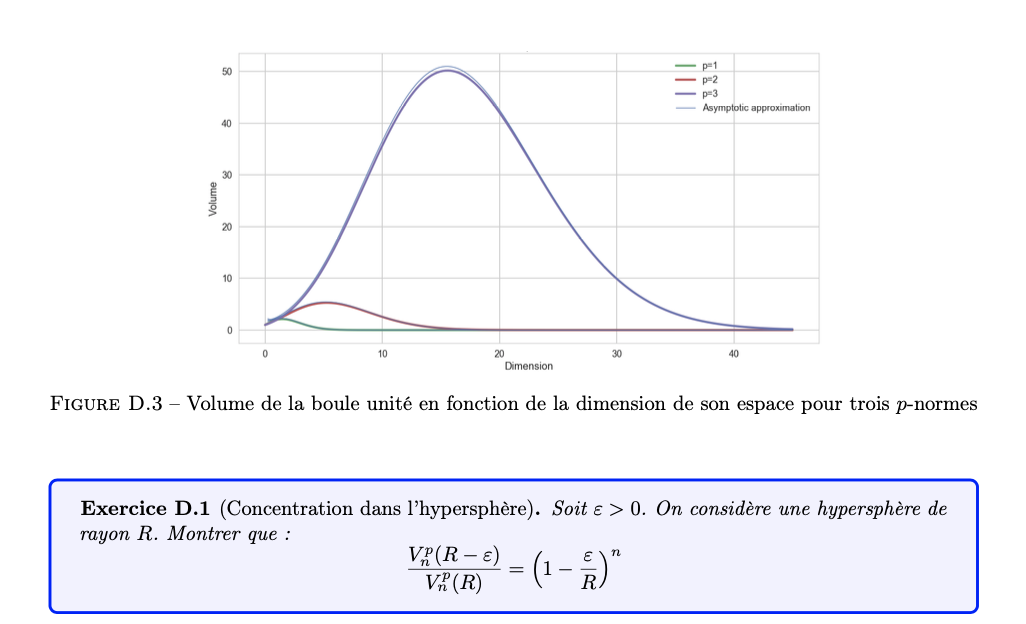
\includegraphics[width=\linewidth]{./img/notions_math/courbe}
\\
On retrouve bien le comportement en hausse que nous avions observé, mais on comprend que le comportement ultime est que le volume tende vers 0 très rapidement. Avant de discuter de ce que ce résultat implique, regardons un autre résultat contre intuitif.
\\
\\
Nous obtenons ici la vérification graphique que nos calculs pour l'approximation semblent corrects. Nous voyons également qu'ils ont la même forme, mais à une échelle très différente. Nous voyons notre premier fait contre intuitif sur la haute dimension : le volume d'une boule de rayon R tendra toujours vers zéro quand la dimension augmentera. La vitesse de convergence dépend à la fois de R et de l'ordre de la norme que nous prenons.
\\
\\
\textbf{Concentration dans l’hypersphère}
\\
Soit $\epsilon$ > 0. On considère une hypersphère de rayon R. Montrer que :
\\
\\
Un autre fait contre intuitif que l'on peut facilement regarder, est que l'essentiel du volume d'une boule est situé dans un minuscule anneau proche de la frontière. En effet, on peut voir que le rapport entre le volume d'une boule de rayon$R-\varepsilon$ et le volume d'une boule de rayon $R$ en dimension $n$ est :
\begin{equation*} \frac{V_n^p(R - \varepsilon)}{V_n^p(R)} = \left(1- \frac{\varepsilon}{R}\right)^n \end{equation*}
C’est encore plus étrange : les points semblent se concentrer proche des frontières de l’hypersphère, donc en ayant un centre vide. Cela veut dire que plus la dimension augmente, plus le volume tend vers 0 et que dans le même temps les données se rapproche des frontières.
\\
Donc si l’on distribue des points uniformément dans une sphère, la distribution des distances entre les points ne sera pas informative du tout. Ces intuitions sont confirmés par la figure ci-dessous.
\\
\\
Toutefois, lorsque $n$ augmente, le ratio converge rapidement vers 0 avec $\varepsilon$ petit. Pour la boule unitaire de dimension $n=100$, 63\% du volume est dans l'anneau de largeur $\varepsilon = 0.01$.
\\
Ensuite, pour la norme euclidienne, si le volume converge vers zéro, mais que la distance maximale entre deux points reste à $2R$ et que la majeure partie du volume est dans un minuscule anneau, la distribution entre les distances par paire ne devrait pas être uniforme même si les points sont tirés au hasard à l'intérieur d'une boule. Nous avons effectué plusieurs tests sur Python :
\\
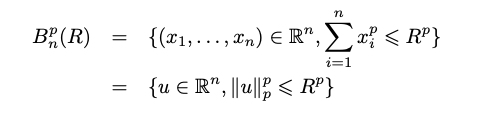
\includegraphics[width=\linewidth]{./img/notions_math/courbe_2}
\\
Ainsi, plus la dimension est grande, moins la notion de distance a du sens. Au delà de l’aspect combinatoire et de stockage des données, avoir un modèle qui a moins d’indicateurs pour s’entraîner aura plus de chance d’être performant et utile. Par exemple, l’ensemble des méthodes de clustering par exemple seront largement impacté par une très grande dimension. Finalement, on peut remettre en cause l’exactitude d’une idée répandue : "Avec plus d’informations les modèles sont meilleurs". Ce qui est plus exact est qu’avec les informations utiles, les modèles sont meilleurs. C’est tout l’enjeux de la phase exploratoire et d’augmentation des données pour répondre à un problème de Machine Learning.
\\
\\
Un deuxième problème majeur en grande dimension est que le nombre de donnée à obtenir pour être capable d’avoir des garanties statistiques sur la qualités de l’apprentissage est colossal, c’est exponentiel. Ainsi, on peut se poser la question de la capacité des algorithmes à apprendre en grande dimension.
\\
\\
Avec cette dernière information, nous comprenons que plus la dimension est élevée, plus les distances sont insignifiantes. Par conséquent, lorsque l'on tente de construire un modèle, il faut toujours rechercher un nombre réduit de variables explicatives et mettre l'accent sur l'utilité des variables. Ce dernier conseil est encore plus important lorsque l'apprentissage automatique est utilisé pour aider d'autres personnes qui ne savent pas ce qu'est l'apprentissage automatique, cela simplifiera grandement l'échange et la collaboration.
\\
\\





\textbf{Interpolation et extrapolation}
\\
\\
L’ensemble du Machine Learning tel qu’on l’a présenté correspond à de l’interpolation et à essayer de faire en sorte que cette interpolation puisse être capable d’extrapoler correctement. Randall Balestriero, Jerome Pesenti et Yann Le Cun on publié en 2021 l’article Learning in High Dimension always amount to extrapolation dont voici le résumé :
\begin{quotation}
    The notion of interpolation and extrapolation is fundamental in various fields from deep learning to function approximation. Interpolation occurs for a sample x whenever this sample falls inside or on the boundary of the given dataset ?s convex hull. Extrapolation occurs when x falls outside of that convex hull. One fundamental (mis)conception is that state-of-the-art algorithms work so well because of their ability to correctly interpolate training data. A second (mis)conception is that interpolation happens throughout tasks and datasets, in fact, many intuitions and theories rely on that assumption. We empirically and theoretically argue against those two points and demonstrate that on any high-dimensional (>100) dataset, interpolation almost surely never happens. Those results challenge the validity of our current interpolation/extrapolation definition as an indicator of generaliza- tion performances.
    \\  
    Randall Balestriero, Jerome Pesenti et Yann Le Cun (2021)
\end{quotation}
L’objet de l’article est de montrer que l’on comprend et défini mal les notions d’interpolation et d’extrapolation en Machine Learning. Cela a des impacts théorique et donc pratique sur notre conception et les garanties mathématiques que l’on peut avoir sur les comportements des algorithmes présenté en très grande dimension. Nous invitons à lire en détail cet article pour en apprendre plus sur le sujet en lui-même, mais également pour voir qu’un domaine qui semble plutôt bien établi et en constante expansion se pose encore des questions sur ses fondements.
\\
\\
En résumé, le fléau de la dimension met en lumière les limites de notre intuition humaine et nous amène à nous questionner encore aujourd’hui sur les fondements communément accepté. Être capable de répondre à ces questions nous permettrait d’être plus précis et plus complet sur notre approche de l’apprentissage en grande dimension.
\\
De manière plus pragmatique, un data scientist doit être au courant que ces questions existent et que le fléau de la dimension va impacter son travail. D’où les techniques de réduction de dimension qui aide à résoudre le problème, mais ne le résolve clairement pas par construction.


    
\newpage






\section{Descente de gradient}
La descente de gradient est une méthode d’optimisation numérique qui s’applique dans de très nombreux domaine. Pour appliquer cette méthode, il faut que nous ayons un problème qui puisse s’écrire sous la forme suivante, avec une fonction $f$ différentiable :
\begin{eqnarray*}
    x^* = \underset{x \in \mathbb{R}^d}{\mathrm{argmin}}\, f(x)
\end{eqnarray*}
Cela ressemble complètement aux différents problèmes que nous avons rencontré jusqu’ici ! La méthode de descente de gradient est une méthode itérative qui va approcher la solution en appliquant la suite :
\begin{eqnarray*}
    x_{t+1} = x_t - \eta \nabla f(x_t)
\end{eqnarray*}
A chaque itération, nous allons nous déplacer dans la direction opposée à la valeur du gradient. Visuellement :
\\
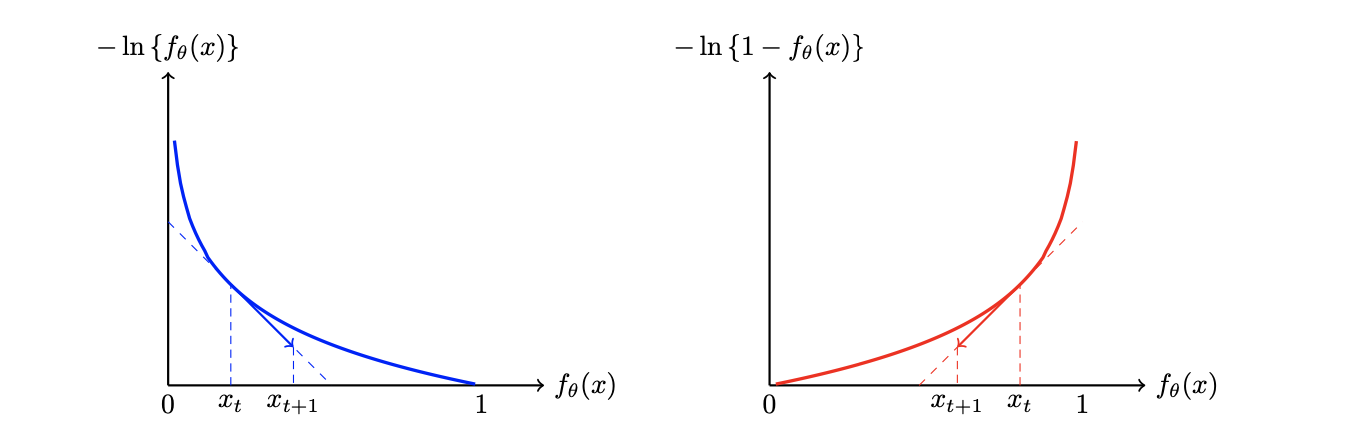
\includegraphics[width=\linewidth]{./img/notions_math/gradiant_descent/courbe_1}
\\
Chaque itération on descend le gradient et l’on s’approche ainsi du minimum de la fonction. Si l’on choisi $x_{t+1}$ comme le point où la tangente croise $y = 0$, alors on obtient l’algorithme de Newton-Raphson qui est également un algorithme d’optimisation. Il est différent de la descente de gradient, car la descente de gradient ne cherche pas à aller jusqu’à $y = 0$ : il va dans cette direction mais parcours $\eta \nabla f(x_t)$ dans cette direction.
\\
\\
En deux dimension, on ne traite plus d’une courbe dont on cherche le minimum comme nous le voyions dans les premiers exemples. On traite ici d’une surface en deux dimensions où l’on cherche les coordonnées du point minimal. Dans la figure (3.2) on voit comment la descente se comporte en plaçant un point à chaque itération.
\\
Le paramètre $\eta$ est crucial dans la descente de gradient, c’est le learning rate. Son rôle est de contrôler l’amplitude des pas de descente. Toujours dans la figure en deux dimensions, on remarque que les points sont de plus en plus rapprochés. La descente de gradient est de moins en moins brusque, et on modifie que très peu le paramètre dans les dernières itérations. Voyons sur l’exemple (3.3) en une seule dimension comment se comporte la descente de gradient en fonction de la valeur de $\eta$.
\\
Le learning rate contrôle la vitesse de convergence vers le minimum (s'il existe), il doit être bien choisit sinon on s’expose à deux problèmes :
\\
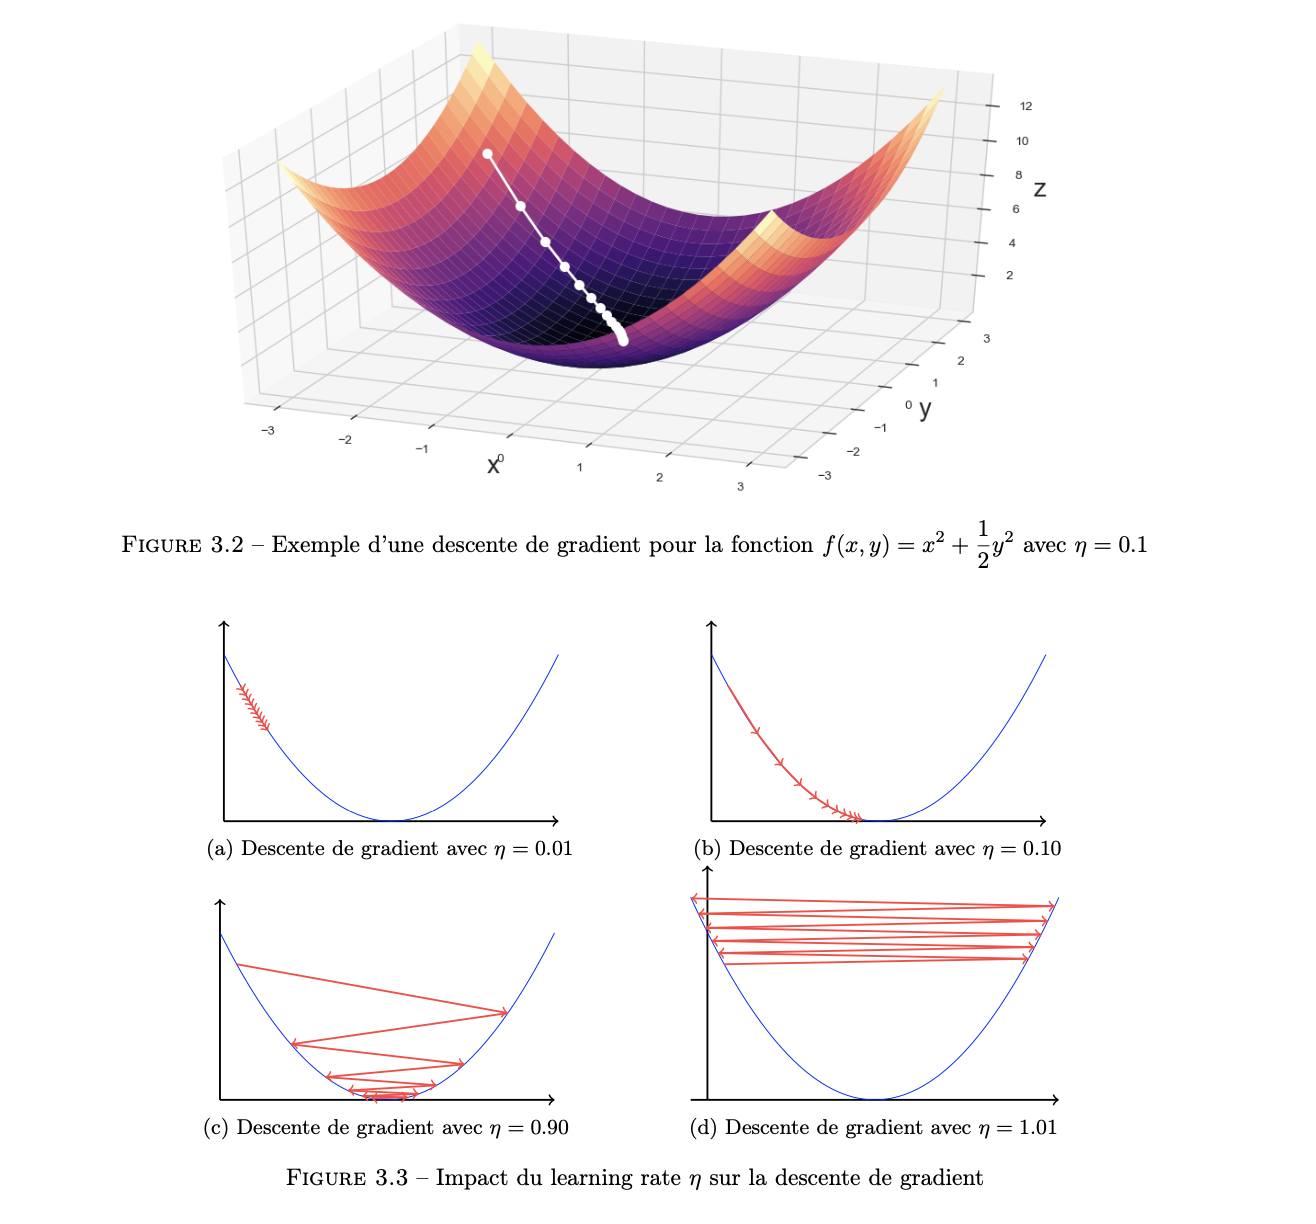
\includegraphics[width=\linewidth]{./img/notions_math/gradiant_descent/courbe_2}
\begin{itemize}
    \item On descend trop doucement : le learning rate est trop faible. C’est le cas de la première descente de gradient (3.3a).
    \item On ne descend pas et on diverge : le learning rate est trop fort. C’est le cas de la dernière descente de gradient (3.3d).
\end{itemize}
La deuxième descente de gradient (3.3b) est parfaite : il y a autant d’itération que pour les autres essais, mais elle converge rapidement vers le minimum que l’on cherche sans avoir à être instable comme (3.3c).
\\
Il n’existe pas de règle universelle pour trouver le learning rate optimal, il s’obtient par de multiple essais empiriques. Il n’est pas non plus obligatoire qu’il soit constant : on peut définir des suites de learning rate par exemple. On peut par exemple vouloir avoir un learning rate fort pour les premières itérations, puis qui réduit progressivement avec le nombre d’itérations.
\\
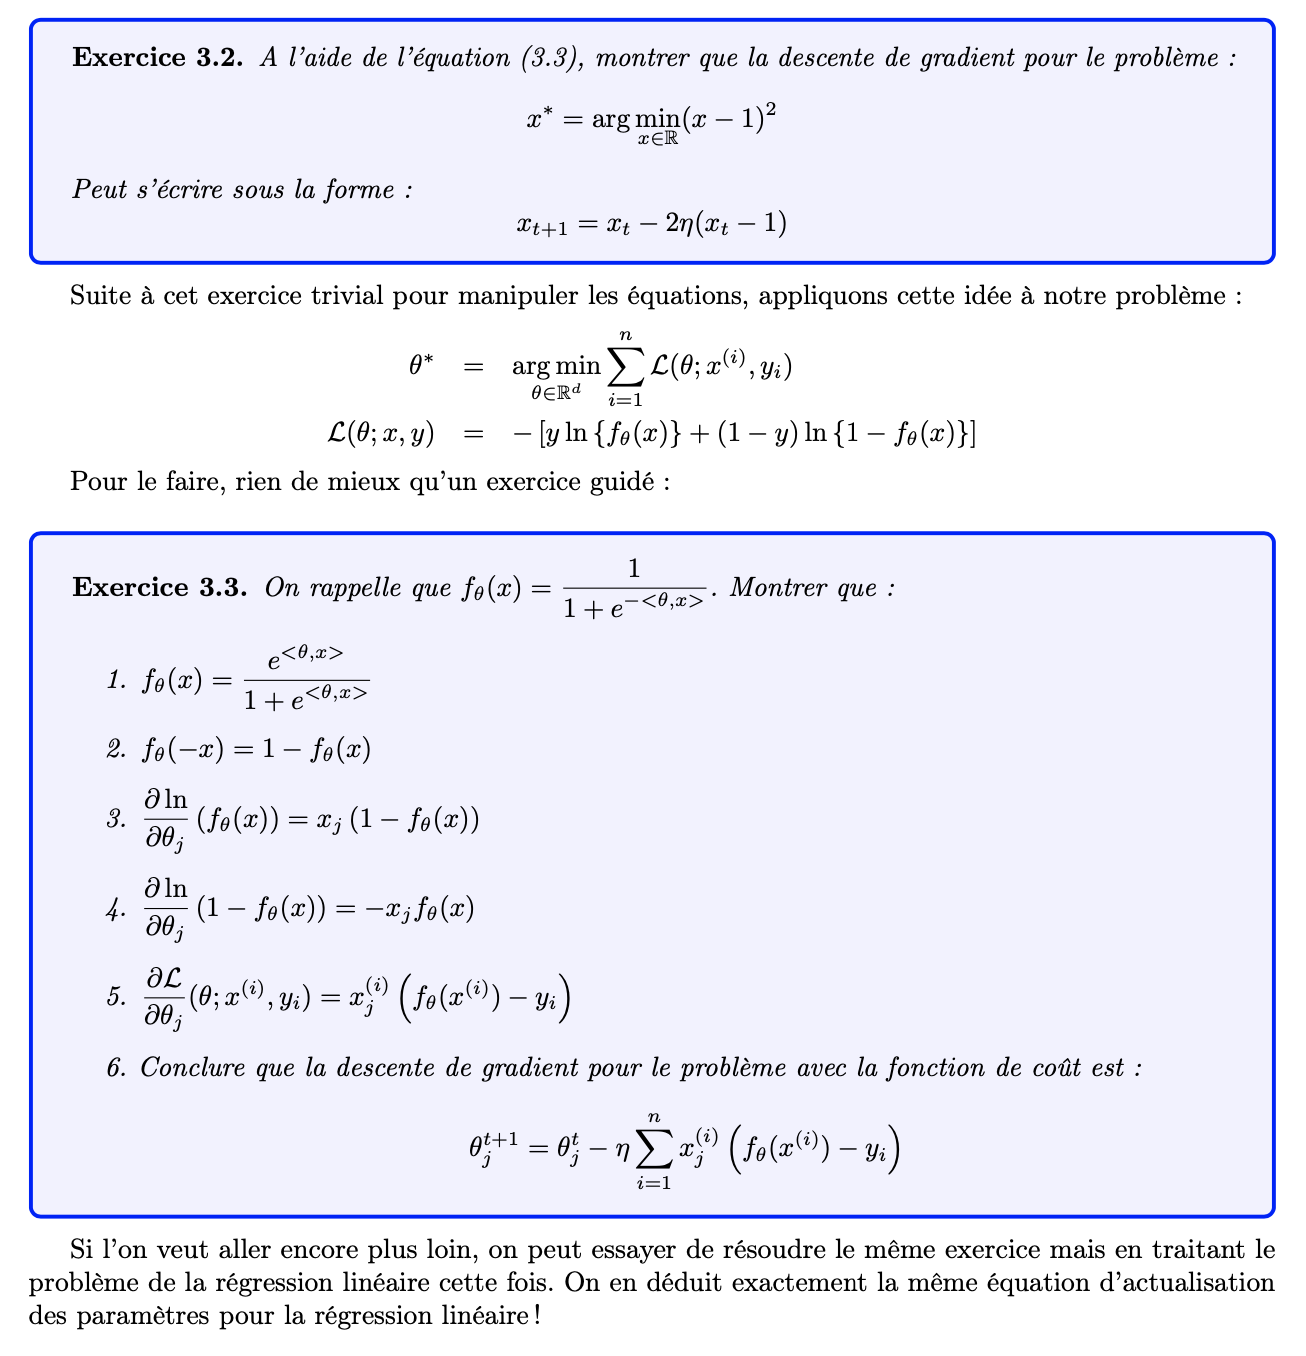
\includegraphics[width=\linewidth]{./img/notions_math/gradiant_descent/exercices}

   % Termine le Chapitre 2
   \newpage
   
%Bibliographie du Chapitre 2
 %  \bibliography{biblio}
   % Termine la biblio du Chapitre 2
   %\newpage

%%%%%%%%%%%%%%%%%%%%%%%%%%%%%%%%%%%%
% Chapitre 3
%%%%%%%%%%%%%%%%%%%%%%%%%%%%%%%%%%%%

% Definition de l'en-tête
\lhead[]{Chapitre 3 : Réduction dimension}
\newpage
   % Inclut fichier tex du Chapitre 3
   \chapter{Réduction dimension}

\section{Cadre théorique}
Calculer une matrice de distance entre chacun des points est un classique de la programmation : trouver le plus court chemin, trouver des observations proches pour une distance, clustering en général... Cette opération essentielle est extrêmement coûteuse en temps de calcul et en mémoire. Pour n observations, nous allons devoir calculer n(n - 1) distances, et ça sera encore pire si la distance est en très grande dimension.


Nous avons donc envie d’être capable de réduire la dimension de l’espace dans lequel on travaille, sans pour autant perdre trop d’informations. Nous y verrons plusieurs approches différentes avec des applications différentes, mais qui partage un but commun : réduire la complexité des données sur lesquelles nous travaillons. Naturellement, nous allons perdre de l’information, et nous verrons comment les différentes méthodes traitent cette minimisation de perte d’informations.


Dans le cadre supervisé nous considérions un dataset composé d’un vecteur et la réponse attendue, mais dans le cadre non supervisé nous n’avons que des observations et aucune réponse. 

\newpage


\section{Johnson-Lindenstrauss}
\subsection{Expliquer puis démontrer le lemme}
La première méthode que nous voyons est à la frontière entre les mathématiques et l’informatique théorique. On comprend dans l’annexe D que plus nous sommes en grande dimension, moins la distance a de sens. Ainsi, nous aimerions tout de même conserver les observations proches dans l’espace de départ dans l’espace d’arrivée. Plus formellement, nous cherchons une fonction f : Rd ! Rk avec k << d telle que pour " > 0 et 8(u, v) 2 D2, nous ayons la propriété :
\\
\begin{equation*} (1-\varepsilon)\|u-v\|_2^2 \leqslant \|f(u)-f(v)\|_2^2 \leqslant (1+\varepsilon) \|u-v\|_2^2 \end{equation*}
\\
Cela ressemble à la définition d’une fonction lipschzienne mais sans coefficient unique de lipschitz. Cela ressemble en réalité plus à une distortion d’ordre au plus 1 + ". Cette similitude est expliqué par le titre de l’article Extension of Lipschitz mapping into a Hilbert space publié en 1984 par William Johnson et Joram Lindenstrauss. Être capable de prouver qu’une telle fonction existe, et dire comment nous pouvons la construire est cruciale. De plus, nous sentons que nous allons avoir une dépendance entre la dimension de l’espace d’arrivée k et la distortion maximale que l’on s’autorise $\varepsilon$. Ce papier répond à toutes ces questions via le lemme suivant.
\\
\\
%\lemme{Soit $\varepsilon>0$ et $\mathcal{D} \in \mathbb{R}^{n\times d}$ un dataset avec $d$ colonnes et $n$ lignes/observations. Si $k > \frac{24}{3\varepsilon^2 - 2\varepsilon^3}\ln{n}$, alors il existe une fonction $f: \mathbb{R}^d \rightarrow \mathbb{R}^k$ telle que :
\\
\begin{equation*} 
(1-\varepsilon)\|u-v\|_2^2 \leqslant \|f(u)-f(v)\|_2^2 \leqslant (1+\varepsilon) \|u-v\|_2^2 
\end{equation*}
pour tout $(u, v) \in \mathcal{D}^2$.


Commençons par observer que la dimension de l’espace de réduction de dépend pas de la dimension de l’espace de départ ! Une manière de saisir pourquoi c’est bien que le cas est que si n > d alors nous pouvons plutôt considérer l’espace engendré par les n observations plutôt que d. Nous sommes bien dans un des pires scénarios, mais la borne sur k tient toujours. Remarquons de plus que le résultat est vrai, peut importe la nature de D, ce qui rend le lemme encore plus général.


Avec le tableau ci-dessous nous pouvons voir les dimensions minimale de l’espace de réduction en fonction de $n$ et $\varepsilon$.


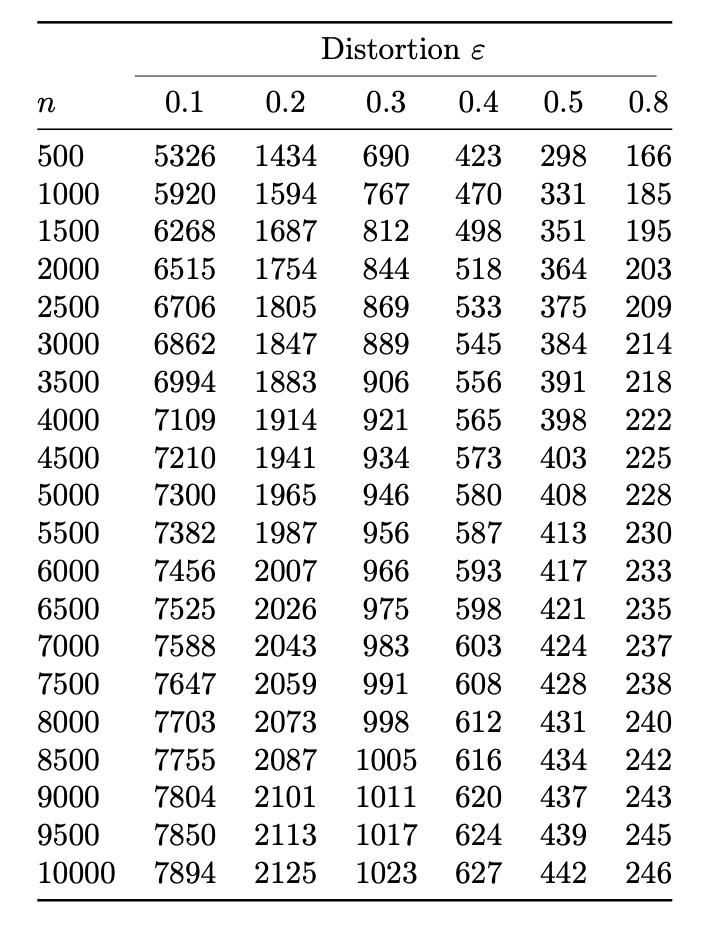
\includegraphics[width=200pt]{./img/reduction_dim/lemme_jl/table}


Nous sentons la progression logarithmique en nombre d’observations : seulement 48\% d’augmentation de l’espace de réduction pour $\varepsilon$ entre n = 500 et n = 10000 qui représente une augmentation de 1900\% en n.
On observe également le comportement prévisible de l’évolution en $\varepsilon$ qui n’est pas linéaire. Etudions un peu plus la valeur de k :


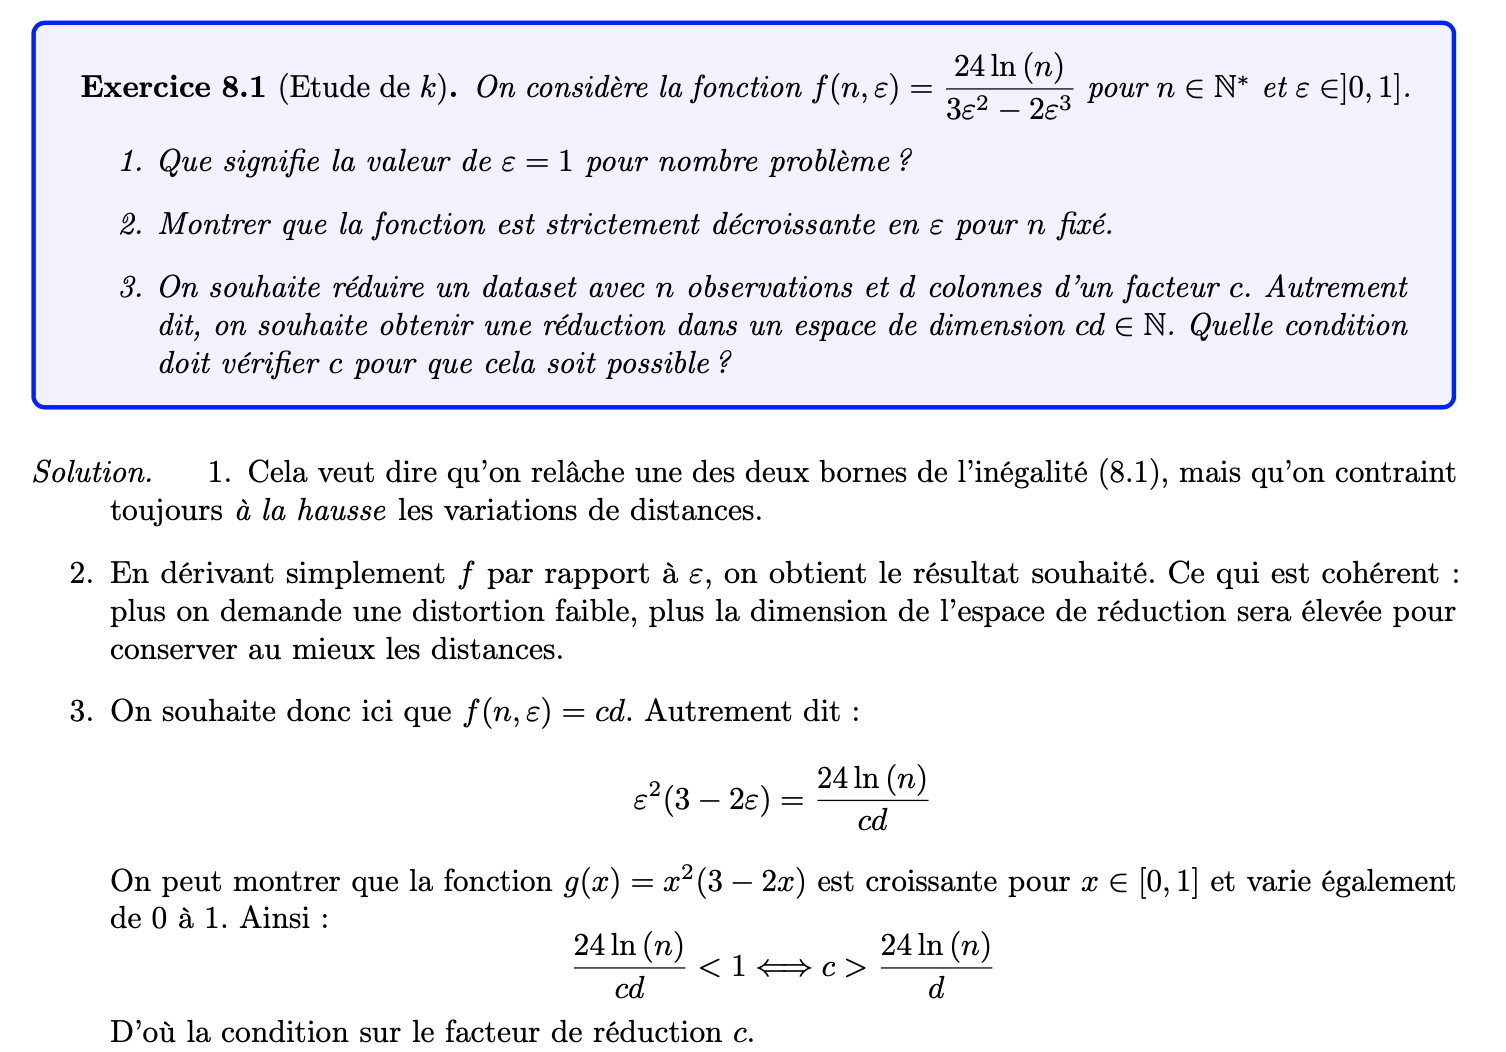
\includegraphics[width=\linewidth]{./img/reduction_dim/lemme_jl/exercice_jl}


Remarquons que le lemme n’est pas toujours avantageux : pour n = 500 et $\varepsilon$ = 0.1, on ne peut pas projeter le dataset dans un espace de dimension plus petit. Pour le faire il faut accepter une distortion d’au moins 0.4.
\\
Avec uniquement le lemme, nous savons qu’une telle fonction existe et quel est la réduction de dimension que l’on peut obtenir. Mais nous ne savons pas comment construire une telle fonction. On obtient la réponse en démontrant le lemme puisque nous pouvons le faire via une démonstration par construction. 
\\
Nous ne le ferons pas ici, mais nous pouvons noter qu’il existe de très nombreuses manière de construire une telle fonction et qu’il s’agit d’un domaine de recherche en informatique.



\includegraphics[width=\linewidth]{./img/reduction_dim/lemme_jl/preuve_1}
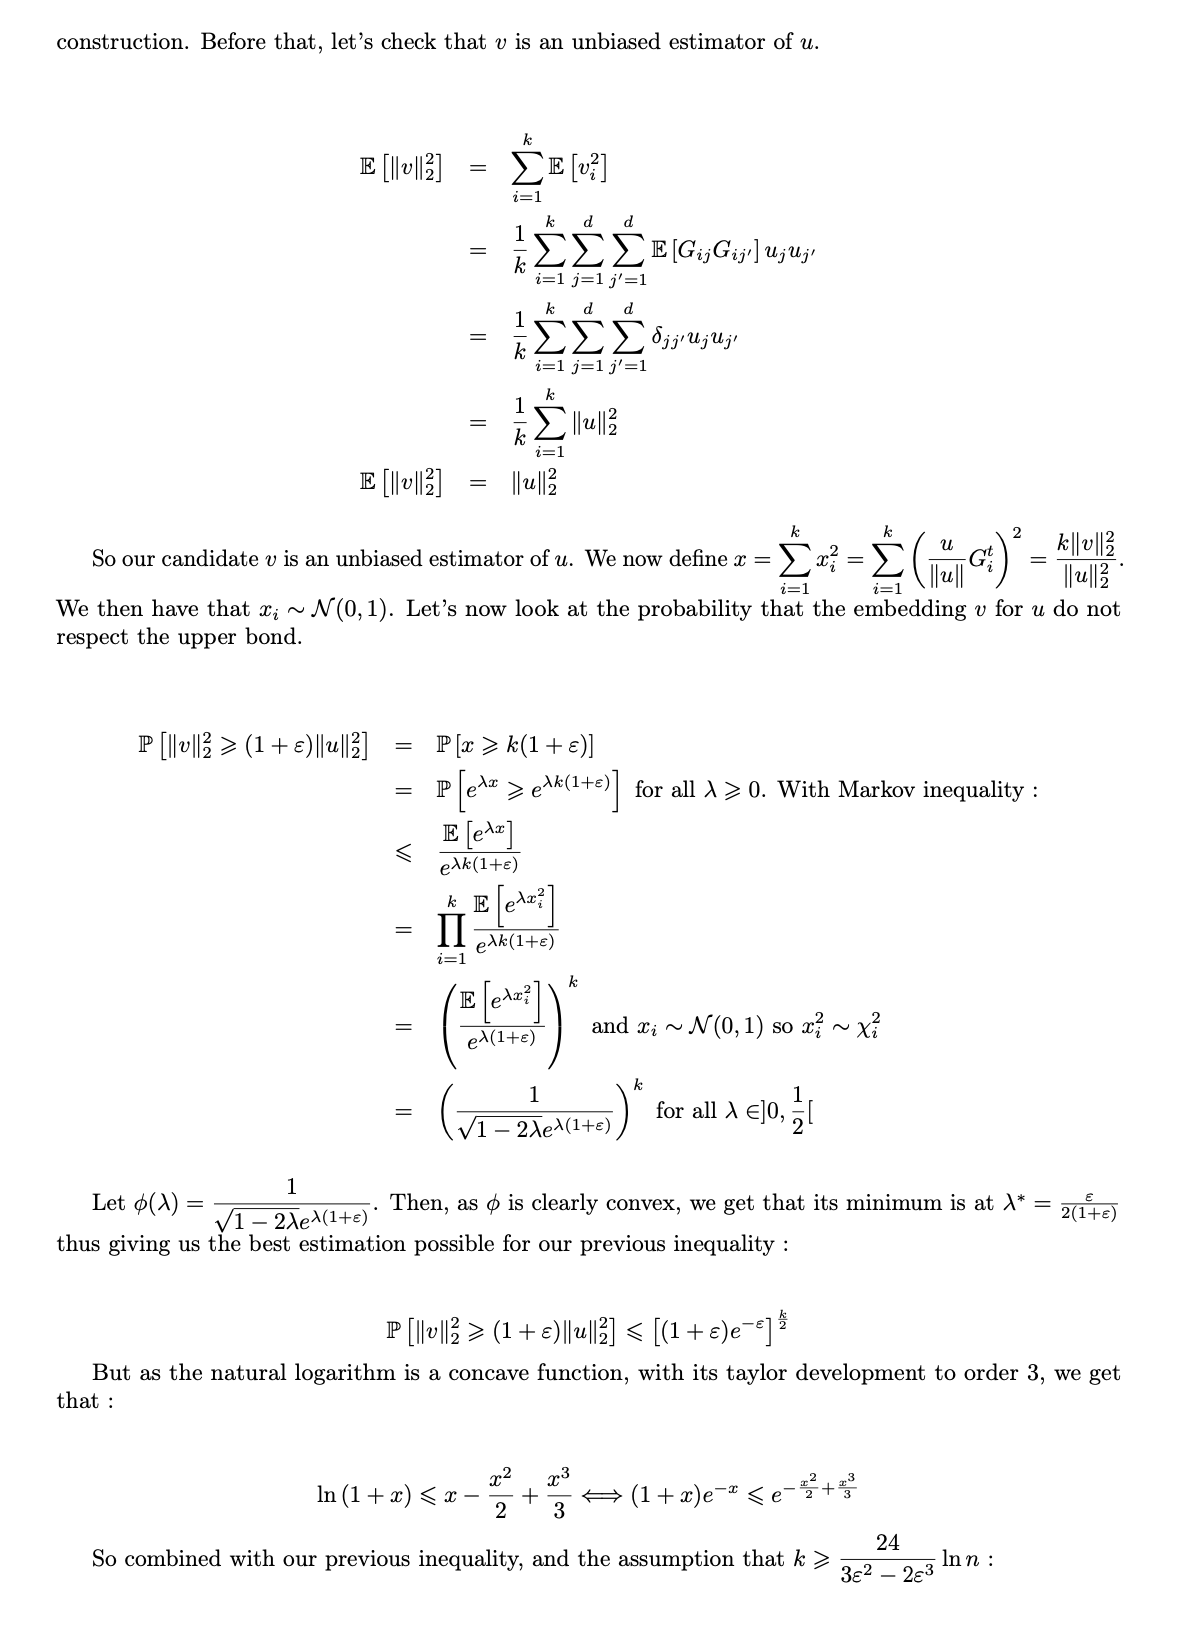
\includegraphics[width=\linewidth]{./img/reduction_dim/lemme_jl/preuve_2}
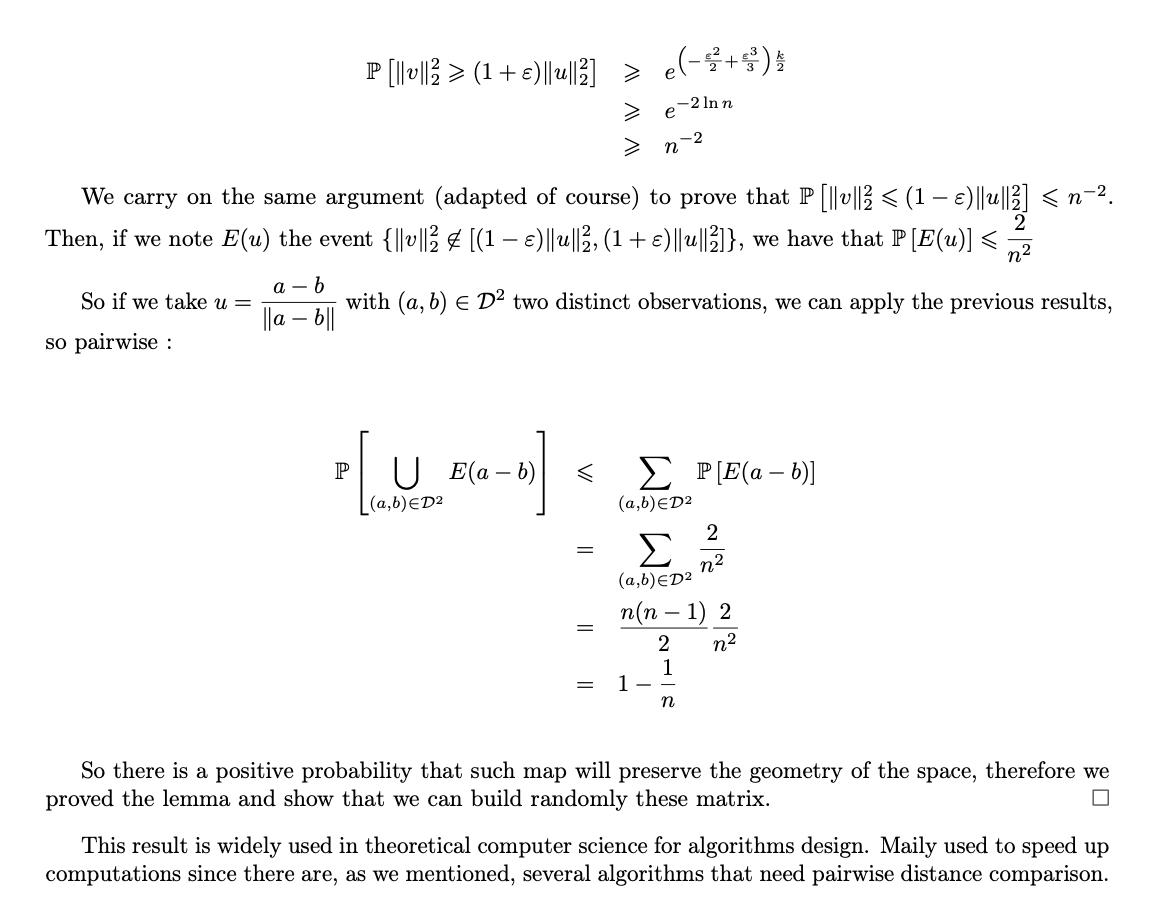
\includegraphics[width=\linewidth]{./img/reduction_dim/lemme_jl/preuve_3}
\\
\\
Ce qui est important de noter, c’est que chacune des preuves de ce résultat construit la fonction f solution en faisant apparaître des projections aléatoire. Autrement dit, en projetant aléatoirement (mais en choisissant bien son aléatoire) dans un espace de dimension k nous pouvons réduire très facilement la dimension de l’espace de départ.
\\
Ce résultat est très largement utilisé en informatique théorique pour le design d’algorithme qui exploitent de très large base de données. Ce résultat est essentiellement utilisé pour accélérer les temps de traitement des algorithmes qui ont besoin de calculer des distances entre chacune des observations de la base.
\\
Les constructions, pour la preuve, peuvent être optimisées pour accélérer encore plus les calculs. Dans la preuve que nous avons faites, nous avons utilisé une matrice dense de variables aléatoire gaussienne : c’est coûteux à la fois en taille et en temps de génération. Dans Database-friendly random projections : Johnson-Lindenstrauss with binary coins, Dimitri Achlioptas montre en 2003 que l’on peut avoir le même résultat avec une matrice avec $\frac{2}{3}$ des entrées vide et uniquement remplie avec des valeurs +1 et -1. C’est bien moins volumineux pour le stockage et rapide à générer.
\\
La meilleure borne a été proposé par Kane Daniel et Nelson Jelani en 2014 dans Sparser Johnson- Lindenstrauss Transforms où la borne ne peut pas être améliorée. En pratique, il y a encore beaucoup de travail sur ce lemme puisque nous n’avons considéré que la distance euclidienne. Si nous travaillons avec la distance manhattan, alors ce résultat ne tient plus. De manière générale pour les normes Lp le résultat n’est pas vrai. Même si la norme euclidienne est de loin la plus utilisée, la norme L1 a plus de sens en grande dimension comme nous l’avons vu avec la régression LASSO.
\\
\\
Pour notre problématique de Machine Learning, ce lemme est utile puisqu’il peut permettre de mieux stocker par exemple des données vidéos, mais il y a plusieurs inconvénients :
\begin{itemize}
    \item La dimension de l’espace de réduction reste élevée pour une visualisation en très petite dimension.
    \item A ce jour, les projections sont faite aléatoirement, donc sans procédure intelligente.
    \item Il n’y a pas de maîtrise du datascientist autre que par le paramètre $\frac{2}{3}$ des projections.
\end{itemize} 
Ces trois points sont pourtant quelque chose que nous souhaiterions obtenir. Il nous faut donc développer d’autre manière de réduire la dimension.


\newpage


        \subsection{Visualiser (un peu)}
        Visualisation


        \newpage













    \section{PCA}
        \subsection{Expliquer la théorie/différence avec Johnson-Lindenstrauss}
            Dans l’analyse par composantes principales il est question d’identifier les directions qui expliquent le mieux les variations des données. Si l’on suppose que les données, par exemple, se distribue uniformément au sein d’une ellipse, nous identifions clairement les axes comme dans la figure ci-dessous :
            \\
            \\
            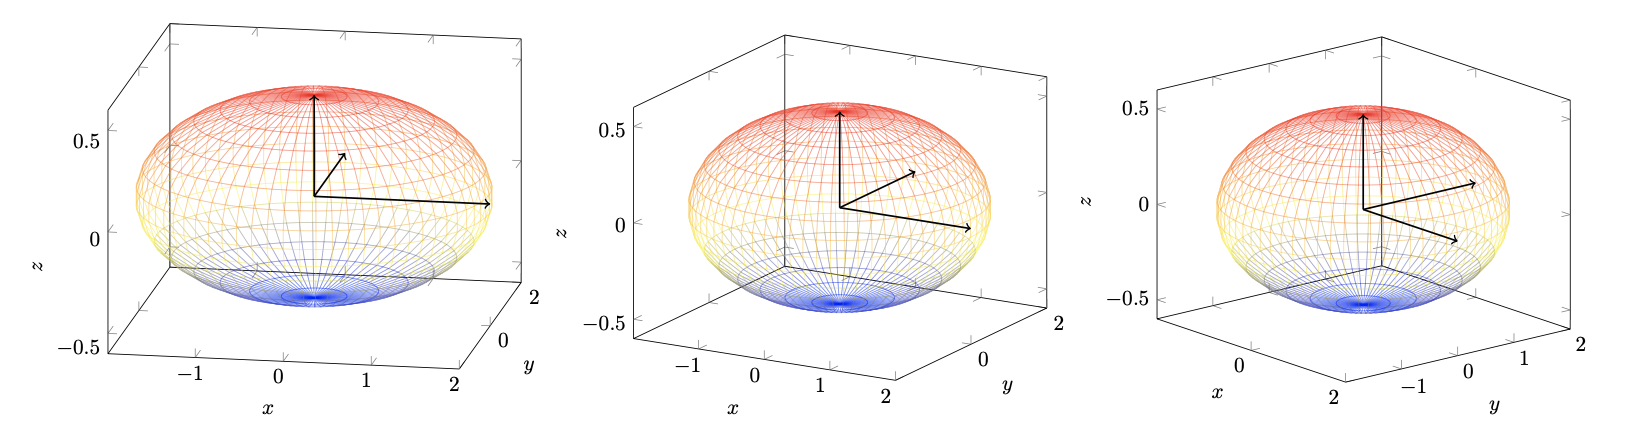
\includegraphics[width=\linewidth]{./img/reduction_dim/pca/elipse}
            \\
            \\
            L’objectif est donc de définir comment trouver ces axes qui nous semblent évident en petite dimension parce que nous sommes capable de les voir, mais cette fois en grande dimension. Si nous sommes capable de les trouver, nous seront en capacité de définir un nouveau repère pour exprimer les informations que nous avons. Ainsi, fort de cette base, nous pourrons sélectionner un échantillon de ses axes pour produire des graphiques compréhensible par l’humain.
            \\
            \\
            Voici les questions auxquelles nous devons répondre :
            \begin{enumerate}
                \item Comment trouver les directions qui décrivent le mieux les variations ?
                \item Comment s’assurer que les directions formeront bien une nouvelles bases ? 
                \item Comment prioriser les directions ?
            \end{enumerate}
            On remarque que les questions ne sont pas toutes bien posées, et nous devons nous laisser guider pour les affiner. Les réponses se trouve dans des notions fondamentales d’algèbre.



                \subsubsection*{Diagonalisation d’une matrice}
                    Soit la matrice $A$ définit comme :
                    \\
                    \begin{eqnarray*}
                         A = \frac{1}{2} \left(\begin{array}{cc}3 & 1 \\ 1 & 3\\\end{array}\right)
                    \end{eqnarray*}
                    \\
                    On sait que si l’on prend un vecteur $u \in \mathbb{R}^2$, on peut multiplier la matrice $A$ par $u$ : on dit en algèbre que $A$ agit sur $u$. Visualisons ce que cela veut dire géométriquement.
                    \\
                    \\
                    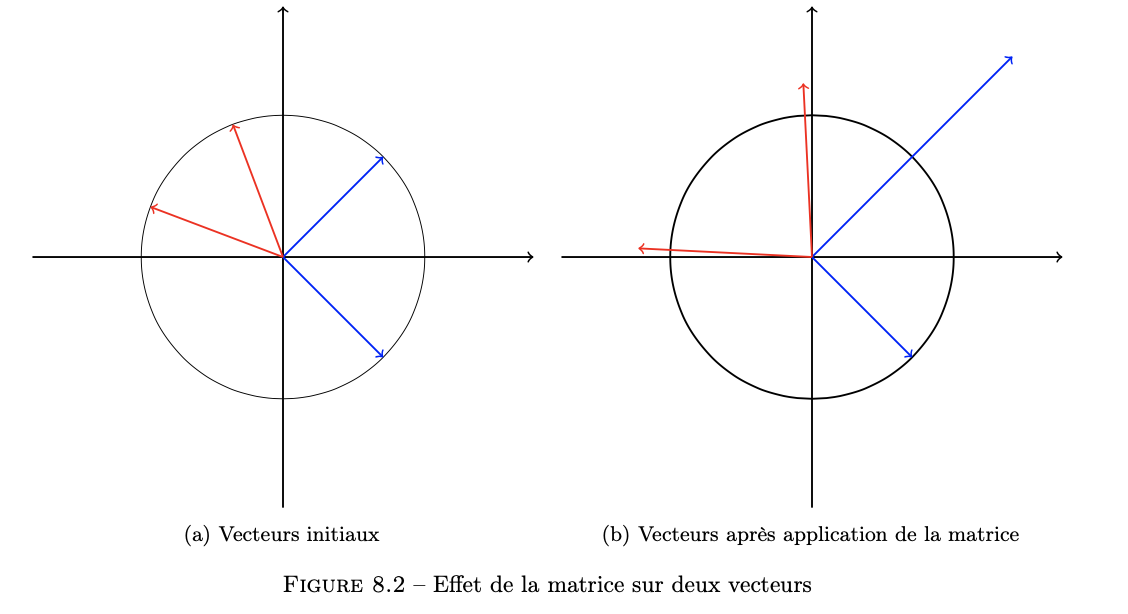
\includegraphics[width=\linewidth]{./img/reduction_dim/pca/vect_prp}
                    \\
                    \\
                    On remarque que les deux vecteurs rouges on changé de direction et de taille, là où les vecteurs bleus ont conservés leurs direction (mais pas nécessairement leurs taille). C’est étonnant d’avoir une invariance de direction pour seulement ces deux directions là (on peut le vérifier par le calcul). Ces deux vecteurs bleus semblent être des vecteurs particuliers pour la matrice A. Généralisons.
                    \\
                    \\
                    On considère une matrice carré A de taille $n$ dans l’ensemble de la section.
                    \\
                    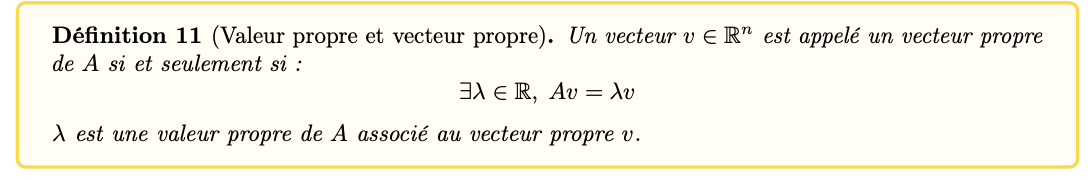
\includegraphics[width=\linewidth]{./img/reduction_dim/pca/def_val_prp}
                    \\
                    Dans notre exemple, le vecteur (1, 1) est un vecteur propre de A ! Et sa valeur propre $\lambda$ est 2. Pour le vecteur (1, -1) sa valeur propre est 1, d’où le non changement d’échelles. Remarquons que si $v$ ne doit pas être nul pour être un vecteur propre, $\lambda = 0$ est autorisé.
                    \\
                    \\
                    Non unicité d’un vecteur propre : soit $\lambda$ une valeur propre de A associé à un vecteur propre $v$. On sait qu’il existe une infinité de vecteur propre lié à la valeur propre $\lambda$.
                    \\
                    Par définition, on a que $Av = \lambda v$, donc si on multiplie par une constante $c \in \mathbb{R}^*$, l’équation devient $cAv = c \lambda v \iff A(cv) = \lambda (cv)$ d’où $cv$ est un vecteur propre de $A$.
                    \\
                    Suite à cette remarque, on comprend que nous n’obtiendrons l’unicité pour un vecteur propre qu’en imposant des règles. Les plus classiques demandes à ce que le vecteur soit de norme 1, mais ça ne garanti par l’unicité encore.
                    \\
                    \\
                    \textbf{Comment trouver les valeurs propres d’une matrice ?}
                    \\
                    (Caractérisation des valeurs propres). $\lambda \in \mathbb{R}$ est une valeur propre de $A$ si et seulement si :
                        $det(\lambda In - A) = 0$
                    \\
                    \\
                    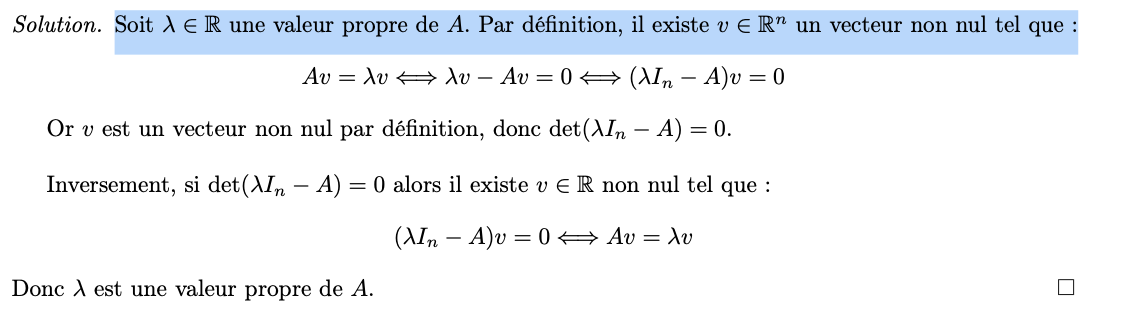
\includegraphics[width=\linewidth]{./img/reduction_dim/pca/prv_val_prp}
                    \\
                    \\
                    Donc $\lambda$ est une valeur propre de $A$.
                    \\
                    \\
                    On appelle l’équation définie dans le théorème (Caractérisation des valeurs propres) l’équation caractéristique de $A$.
                    \\
                    Le polynôme en $\lambda$ issue de cette équation est de degré au plus $n$, et donc nous sommes certains d’avoir $n$ racines complexes, potentiellement complexes et potentiellement répétées. Ici, nous avons donc bien nos deux vecteurs bleus qui sont les seuls vecteurs propres de la matrice $A$ de l’exemple.
                    \\
                    \\
                    Maintenant que nous sommes capables de trouver l’ensemble des valeurs propres d’une matrice, en résolvant l’équation $Av = \lambda v$ en $v$ et en sélectionnant les vecteurs propres de norme 1, nous sommes également capable de calculer l’ensemble des vecteurs propres.
                    Un résultat (que nous ne démontrerons pas) nous informe que cette ensemble de vecteur propre forme une base, autrement dit, les vecteurs sont de norme 1 et orthogonal entre eux. Ainsi, on définit :
                    \\
                    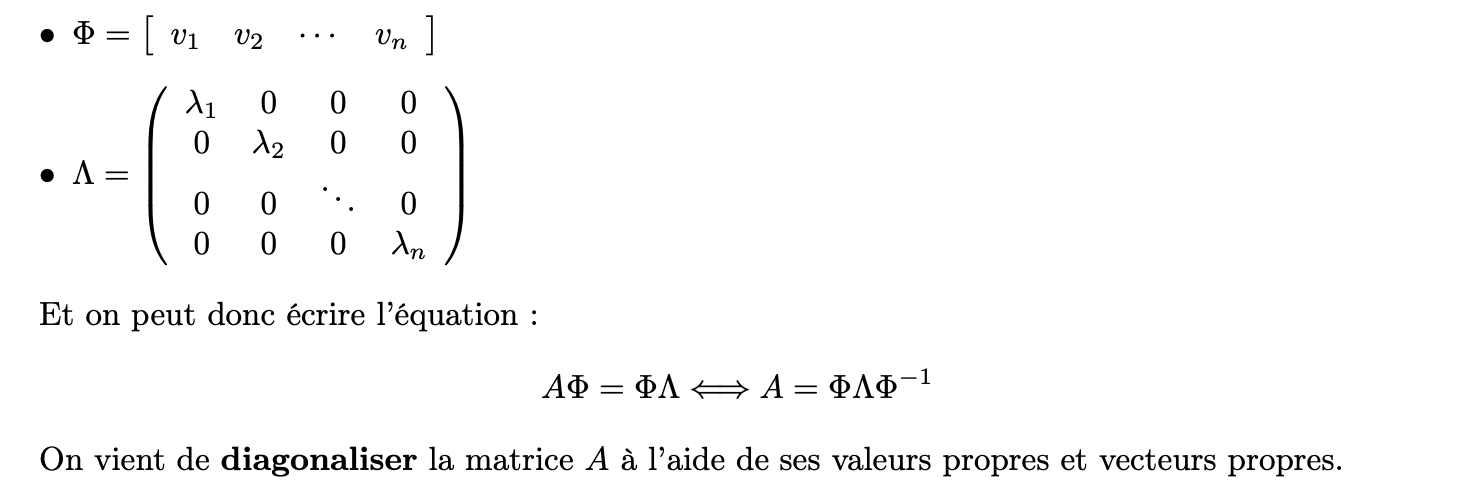
\includegraphics[width=\linewidth]{./img/reduction_dim/pca/mat_diag}
                    \\
                    \\
                    \textbf{(Puissance d’une matrice) Soit A une matrice diagonalisable de taille d. Calculer $A^n \in \mathbb{N}$ :}
                    \\
                    Puisque $A$ est diagonalisable, il existe $\Phi$ et $\Lambda$ défini comme précédemment telle que $A = \Phi \Lambda \Phi^{-1}$. Par récurrence rapide, on peut montrer que :
                    \\
                    
\includegraphics[width=\linewidth]{./img/reduction_dim/pca/mat_puissance}
                    \\
                    C’est un résultat qui permet d’accélérer très nettement les calculs de puissance de matrice puisque nous n’avons besoin de calculer que deux multiplications de matrice, au lieu de $n$. Mais on pourrait se dire que calculer l’inverse de la matrice $\Phi$ coûte. En pratique, comme nous avons une base, $\Phi^{-1} = \Phi^t$.
                    \\
                    \\
                    Voyons sur un exemple comment l’analyse par composante principale nous permet de mieux visualiser une matrice :
                    \\
                    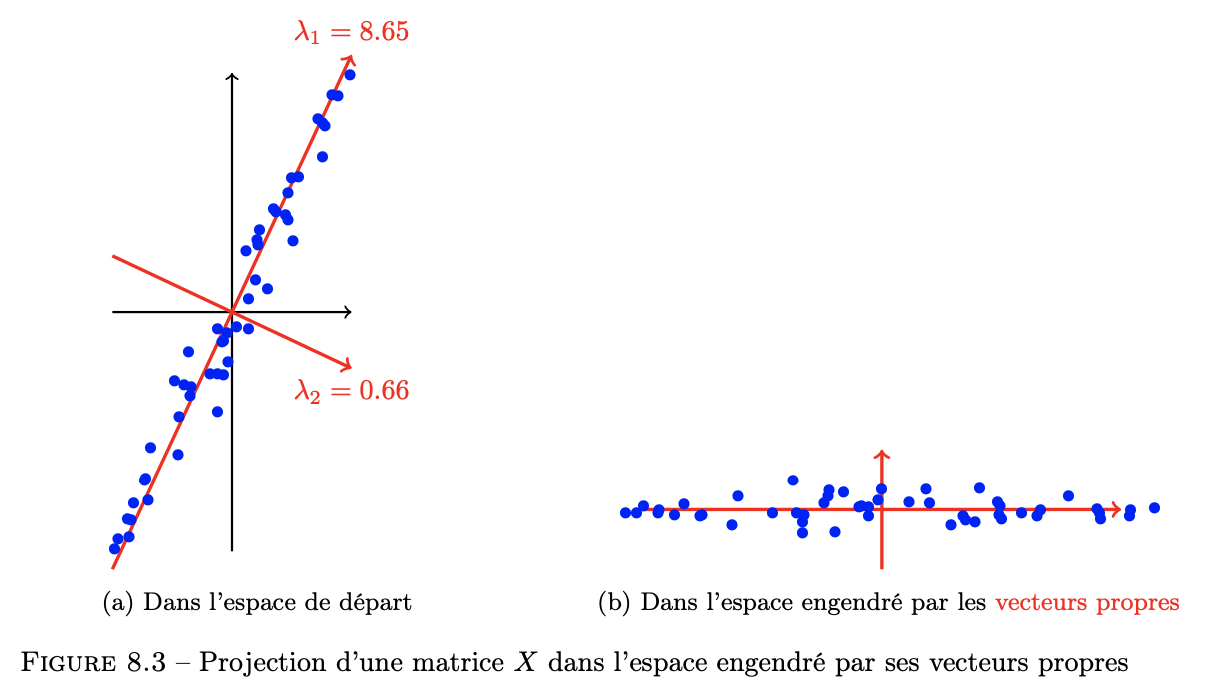
\includegraphics[width=\linewidth]{./img/reduction_dim/pca/graph_mat}
                    \\
                    Dans la figure ci-dessus, on présente la projection de l’espace de départ (engendré par $X$) et l’espace défini par les vecteurs propres de $X$. C’est exactement ce que l’on voulait : le grand axe de variation a été comprit, et les deux vecteurs propres forment une base orthonormée pour projeter $X$. Ainsi, on peut se suffire de la composante liée à $\lambda_1$ pour bien approcher les variations de la matrice : on a bien réduit la dimension.



                \subsubsection*{Application à la réduction de dimension}
                    C’est cette dernière remarque qui motive notre utilisation de ces résultats d’algèbre. Nous pouvons projeter $X$ dans un sous-ensemble de ses vecteurs propres et conserver a priori le plus de variations expliquées. Se posent alors deux questions :

                    \begin{enumerate}
                        \item Est-t-on certain que l’on pourra toujours diagonaliser X ?
                        \item Comment prioriser les composantes à conserver ?
                    \end{enumerate}

                    La première question est répondu par la négative : il n’y a aucune garantie mathématiques qu’une matrice quelconques puissent être diagonalisable. $X$ n’est même pas une matrice carré en règle général ! Puisqu’on cherche à identifier les axes où la variance est la plus forte, décomposons la matrice de variance-covariance de $X$ ! On la note $\Sigma $et dans notre cas, elle se définit comme :
                    \\
                    \\
                    \begin{eqnarray*}
                        \Sigma = \frac{XX^t}{n - 1}
                    \end{eqnarray*}
                    \\
                    \\
                    Chaque coefficient $(\sigma_{ij})_{1 \leqslant i, j \leqslant d}$ de $\Sigma$ représente la covariance entre l’information $i$ et l’information $j$. Ainsi, quand $i = j$, cela revient à avoir la variance de l’information $i$, d’où le nom de matrice de variance-covariance. Cela fait déjà plus de sens philosophiquement, et on a cette fois la garantie de toujours pouvoir la diagonaliser puisque $\Sigma$ est une matrice symétrique semi-définie positive.
                    \\
                    \\
                    Il reste à savoir comment prioriser les composantes à conserver. On remarque dans la figure (8.3) que les valeurs propres associées à chacun des axes sont très différentes et on dirait que la valeur est corrélées à l’importance de la direction.
                    Voyons avec un exercice comment nous pouvons tirer partie de cette information.
                    \\
                    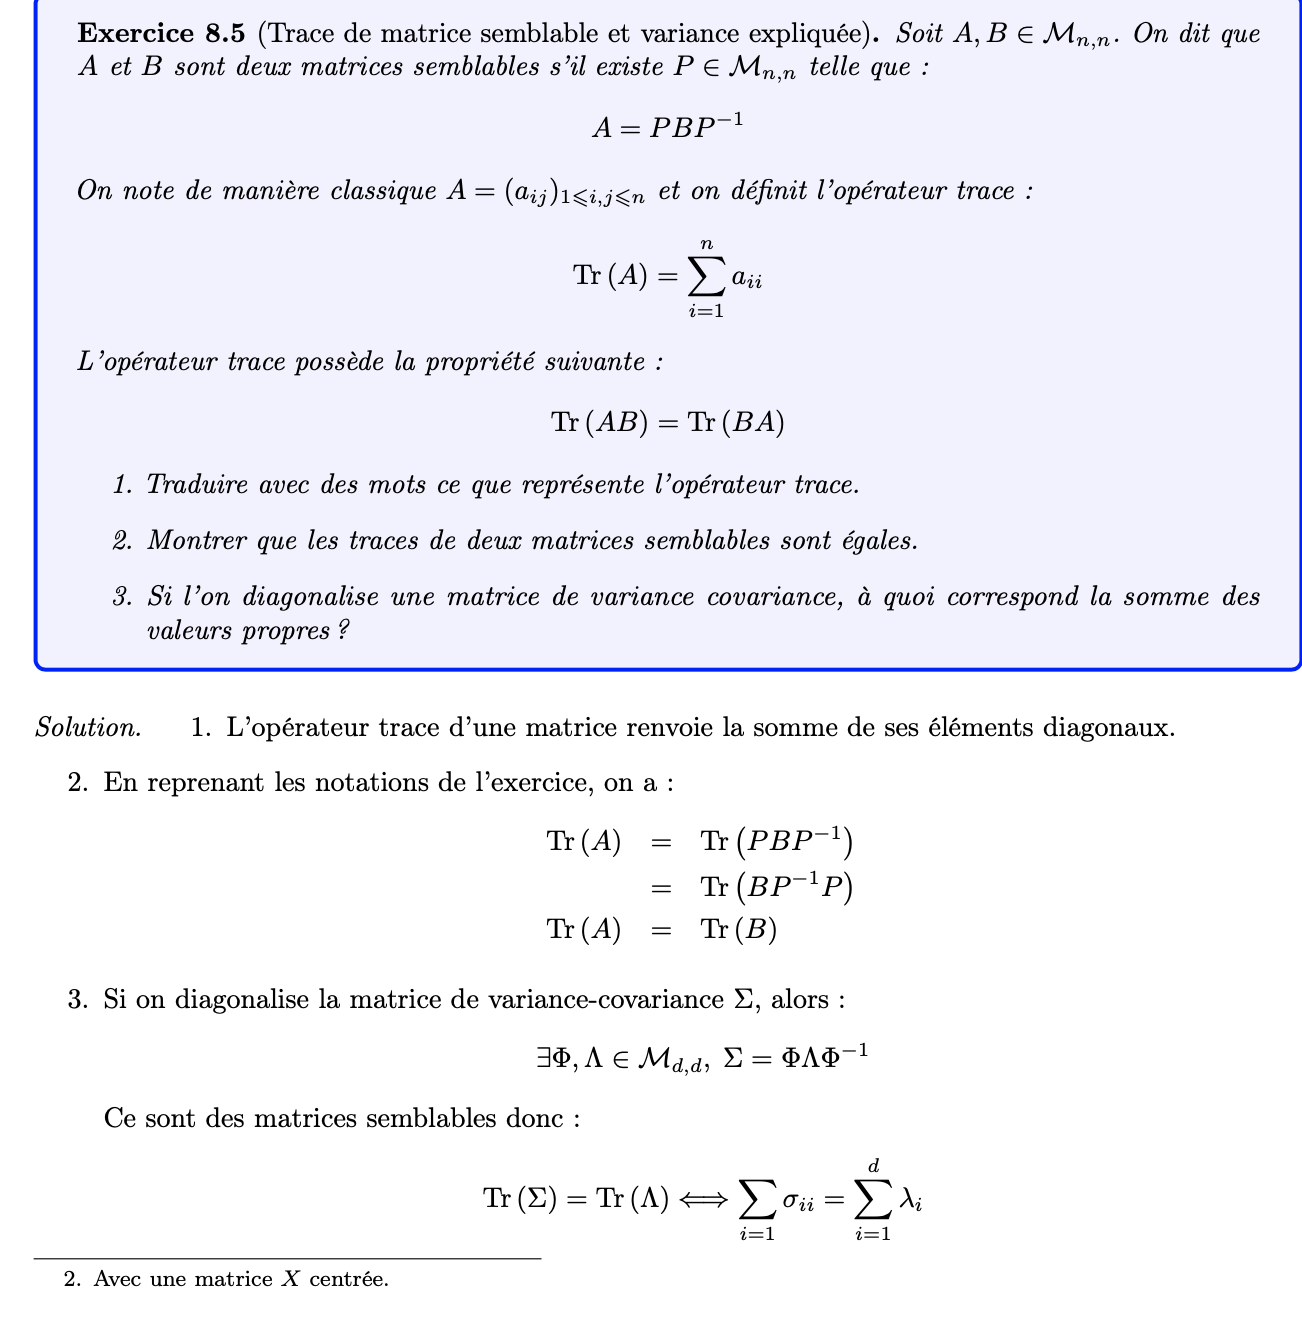
\includegraphics[width=\linewidth]{./img/reduction_dim/pca/mat_trace}
                    \\
                    Autrement dit, la somme des variances de chacune des informations contenues dans la matrice $X$ est égale à la somme des valeurs propre de la matrice de variance-covariance.
                    \\
                    \\
                    Avec cet exercice on comprend comment nous allons prioriser les axes à conserver : plus une valeur propre est grande, plus sa composante associée est importante. De plus, nous sommes capable de définir la proportion de variance expliquée par chacune des composantes.
                    \\
                    Par exemple, dans la figure (8.3), la première composante explique 93\% de la variance. D’où notre intuition de dire qu’il suffisait de conserver uniquement la première composante pour mieux visualiser les données.
                    \\
                    \\
                    Par rapport au lemme de Johnson-Lindenstrauss, cette fois nous sommes capable d’expliquer chacun des axes créés avec une procédure intelligente. En revanche, nous faisons l’hypothèse que les variations peuvent être expliquées par une combinaison linéaire des informations présentes, ce qui n’est pas forcément le cas.
                    \\
                    \\
                    Finalement, l’analyse par composante principale cherche à résumer la forme de la matrice avec une vision macro via une explication de la variance. Que faire si nous souhaitons réduire la dimension en conservant une vision plus micro cette fois ?


        \newpage





        \subsection{Visualisation}
        Visualisation


        \newpage








    \section{Nouvelle approche : t-SNE}
        \subsection{Cadre théorique}
        T-Distributed Stochastic Neighbor Embedding (t-SNE) a été développé par Laurens van der Maaten et Geoffrey Hinton en 2008. La principale différence avec PCA est que t-SNE est un algorithme de réduction de dimension non linéaire. Ce que cela signifie, c'est que cet algorithme permet de séparer des données qui ne peuvent être séparées par des lignes droites.
        \\
        \\
        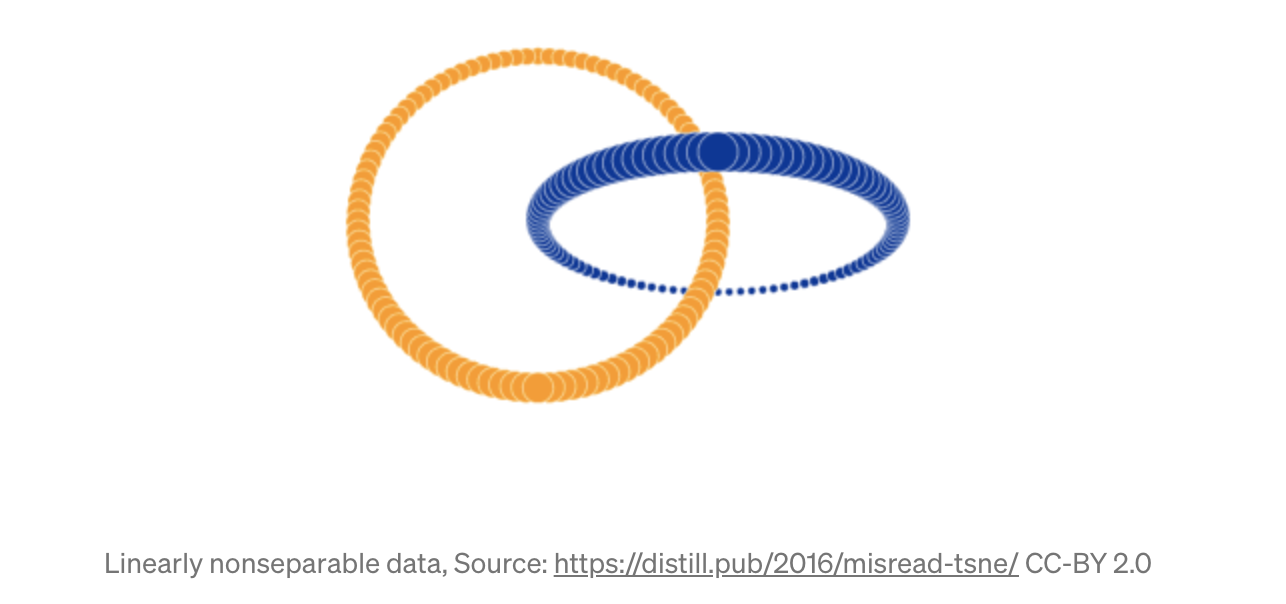
\includegraphics[width=\linewidth]{./img/reduction_dim/t_sne/exemple_data}
        \\
        \\
        Comme le montre cet exemple, il n'est pas possible de séparer ces données de manière linéaire. C'est pour cela que l'utilisation de t-SNE est pertinente dans ce cas précis comparé à PCA.
        \\
        \\
        Ici, la descente de gradient est utilisée pour réduire le graphe en faible dimension dans lequel la distance relative entre les points i et j correspond à celle de l'espace original de haute dimension ; sous le contrôle d'un paramètre de perplexité qui détermine l'écart-type des distributions conditionnelles utilisées pour les calculs de distance relative dans l'espace de haute dimension. Cette méthode se concentre principalement sur la structure locale, elle met l'accent sur les plus proches voisins dans les calculs de distance relative.
        \\
        \\
        Nous allons voir plus précisément comment t-SNE fonctionne :



            \subsubsection*{Distribution de probabilités}
            La première partie de l'algorithme consiste à créer une distribution de probabilité qui représente les similarités entre voisins. L'article original décrit la similarité comme étant " la similarité du point de données $x_j$ au point de données $|x_i-x_j|$ est la probabilité conditionnelle $p_{j|i}$, que $|x_i-x_j|$ choisisse $x_j$ comme voisin".
            \\
            \\
            On choisi un des points du jeu de données. Maintenant, nous devons choisir un autre point et calculer la distance euclidienne entre eux $|x_i-x_j|$. L'article original indique qu'elle doit être proportionnelle à la densité de probabilité sous une gaussienne centrée sur $x_i$. Nous devons donc générer une distribution gaussienne avec une moyenne à $x_i$, et placer notre distance sur l'axe des X. 
            \\
            Après avoir calculé cette première distance, nous devons faire la même chose pour toutes les distances avec chaque point. 

                

            \subsubsection*{Clusters dispersés et variance}
            Maintenant que nous avons effectué l'étape précedente pour tous les points du premier cluster, nous faisons la même chose pour le/les suivants.
            \\
            \\
            Lorsque l'on a fait l'oppération pour tous les points (de tous les clusters), on peut distinguer les points similaires (et non similaires). Mais on peut aussi remarquer que les valeurs absolues des probabilités sont beaucoup plus faibles ou plus importantes que dans d'autres cluster.
            \\
            Nous corrigeons cela en divisant la valeur de la projection actuelle par la somme des projections : 
            \\
            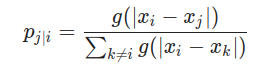
\includegraphics[width=100pt]{./img/reduction_dim/t_sne/eq_prob_1.png}
            \\
            Cela met à l'échelle toutes les valeurs pour que leur somme soit égale à 1. Il est important de remarquer que $p_{i|i}$ est évidement fixé à 0 et non à 1.

            
            \subsubsection*{Gérer des distances différentes}
            Si nous prenons deux points et essayons de calculer la probabilité conditionnelle entre eux, les valeurs de $p_{i|j}$ et $p_{j|i}$ seront possiblement différentes. En effet, elles proviennent de deux distributions différentes. Laquelle devons-nous donc choisir pour le calcul ?
            \\
            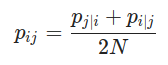
\includegraphics[width=100pt]{./img/reduction_dim/t_sne/eq_prob_2.png}
            \\
            Avec N le nombre de dimensions.
            \\
            \\
            Ainsi, nous avons tout mis à l'échelle de 1, la somme de tout est égale à 1. Mais nous avons ici simplifié la formule pour comprendre plus facilement comment cela focntionne, la formule originale dans le papier de recherche est la suivante : 
            \\
            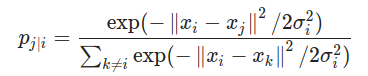
\includegraphics[width=100pt]{./img/reduction_dim/t_sne/eq_prob_3.png}
            \\







\subsubsection*{Perplexité}
En regardant cette formule, on remarque que :
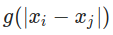
\includegraphics[width=100pt]{./img/reduction_dim/t_sne/eq_prob_4.png}
\\
équivaut à 
\\
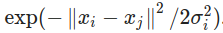
\includegraphics[width=100pt]{./img/reduction_dim/t_sne/eq_prob_5.png}
\\
Nous avons simplifié, car il serait difficile d'expliquer d'où vient $\sigma^2$ et quelle est la dépendance entre lui et nos clusters. On sait que la variance dépend de la gaussienne et du nombre de points entourant le centre de celle-ci. C'est ici qu'intervient la valeur de perplexité.
\\
La perplexité est plus ou moins un nombre cible de voisins pour notre point central. Fondamentalement, plus la perplexité est élevée, plus la variance a une valeur élevée. 
\\
Selon le papier original : "SNE effectue une recherche binaire de la valeur de sigma qui produit une distribution de probabilité avec une perplexité fixe qui est spécifiée par l'utilisateur".
\\

\includegraphics[width=100pt]{./img/reduction_dim/t_sne/eq_prob_6.png}
\\
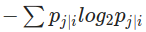
\includegraphics[width=100pt]{./img/reduction_dim/t_sne/eq_prob_7.png}
\\
C'est l'entropie de Shannon. La principale chose que l'on doit savoir est que la perplexité que l'on choisit est positivement corrélée avec la valeur de $\mu_i$ et pour la même perplexité, vous aurez plusieurs $\mu_i$ différents, basés sur les distances. La valeur de perplexité typique se situe entre 5 et 50.
\\
\\
\textbf{Intérpretation de la formule originale}
\\
\\
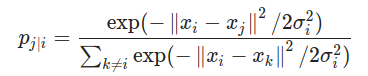
\includegraphics[width=100pt]{./img/reduction_dim/t_sne/eq_prob_8.png}
\\
Lorsque vous regardez cette formule, vous pouvez remarquer que notre gaussienne est convertie en : 
\\
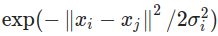
\includegraphics[width=100pt]{./img/reduction_dim/t_sne/eq_prob_9.png}
\\
Cela permet de distinguer les probabilités du voisin.





\subsubsection*{Créer un espace de faible dimension}
La partie suivante de t-SNE consiste à créer un espace de faible dimension avec le même nombre de points que dans l'espace original. Les points doivent être répartis de manière aléatoire dans le nouvel espace. 
\\
Le but de cet algorithme est de trouver une distribution de probabilité similaire dans l'espace à faible dimension. Le choix le plus évident pour la nouvelle distribution serait d'utiliser à nouveau les gaussiennes. Ce n'est malheureusement pas la meilleure idée. L'une des propriétés de la gaussienne est qu'elle a une "queue courte", ce qui crée un problème d'encombrement.
\\
Pour résoudre ce problème, nous allons utiliser la distribution t de Student avec un seul degré de liberté. Nous ne développerons pas notre choix ici par souci de simplicité, afin de se concentrer sur l'essentiel.
\\
Nous obtenons donc :
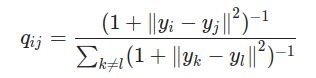
\includegraphics[width=100pt]{./img/reduction_dim/t_sne/eq_red_dim_1.png}
\\
Au lieu de :
\\
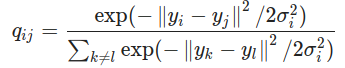
\includegraphics[width=100pt]{./img/reduction_dim/t_sne/eq_red_dim_2.png}
\\
Visuellment cela donne : 
\\
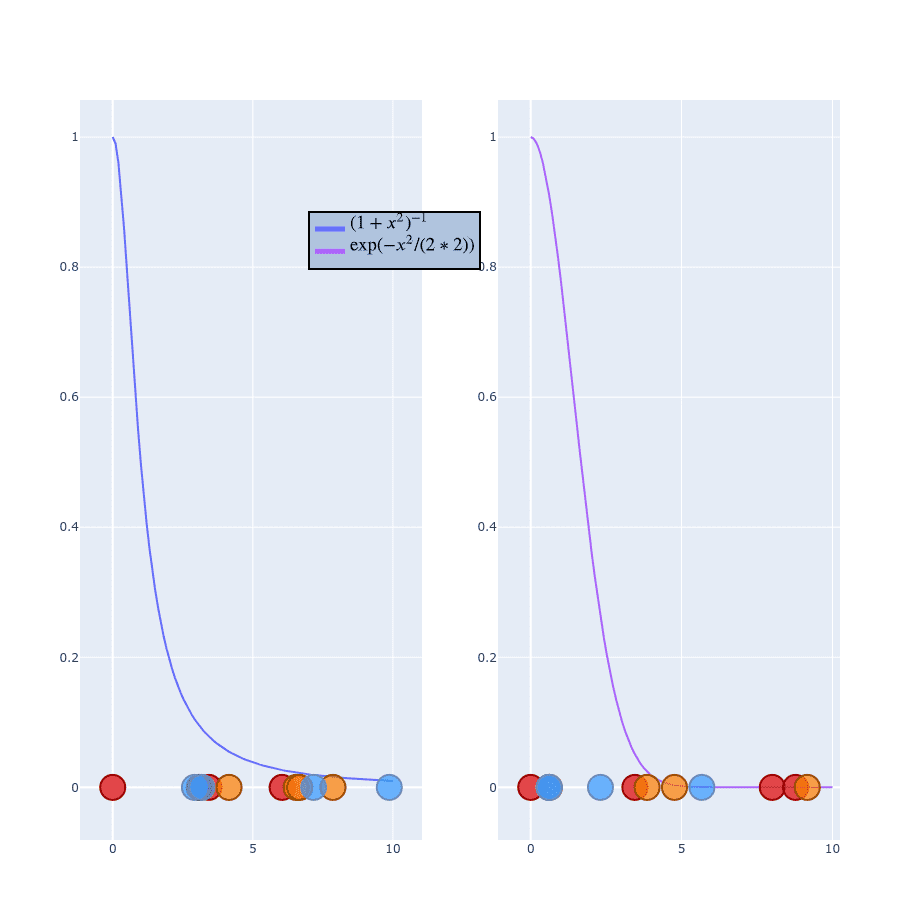
\includegraphics[width=\linewidth]{./img/reduction_dim/t_sne/graph.png}
\\
L'utilisation de la distribution de Student résout notre problème. Elle "tombe" rapidement et a une "longue queue", de sorte que les points ne seront pas écrasés en un seul point.
\\
Cette fois, nous n'avons pas à nous soucier de $\sigma^2$, car il n'y en a pas dans la formule de $q_{ij}$. Nous n'allons pas générer tout le processus de calcul de $q_{ij}$ car il fonctionne exactement de la même manière que $p_{ij}$. Voici les deux formules et passons à la suite :
\\
\includegraphics[width=\linewidth]{./img/reduction_dim/t_sne/eq_red_dim_3.png}
            





\subsubsection*{Déscente de gradient}
Pour optimiser cette distribution, t-SNE utilise la divergence de Kullback-Leibler entre les probabilités conditionnelles $p_{j|i}$ et $q_{j|i}$ :
\\
\includegraphics[width=\linewidth]{./img/reduction_dim/t_sne/desc_grad_1.png}
\\
Nous n'allons pas faire le calcul ici. Ce dont nous avons besoin, c'est de la dérivée :
\\
\includegraphics[width=\linewidth]{./img/reduction_dim/t_sne/desc_grad_2.png}
\\
Le gradient agit comme une répulsion et une attraction entre les points. Un gradient est calculé pour chaque point et décrit la "force" avec laquelle il doit être attiré et la direction qu'il doit choisir.
\\
\\
C'est une exagération t-SNE n'est pas aussi rapide. Nous avons sauté beaucoup d'étapes pour simplifier la compréhansion du processus.
\\
\\
Si l'on reprend les données de notre introduction, voici une résolution possible de t-SNE : 
\\
\includegraphics[width=\linewidth]{./img/reduction_dim/t_sne/exemple_data}
\\
\includegraphics[width=\linewidth]{./img/reduction_dim/t_sne/exemple_data_2.png}
            


\subsubsection*{Conclusion}
Ici, nous avons vu que t-SNE distribue les clusters uniformément autour du centre, ce qui contribue à préserver la structure locale, mais au détriment d'informations sur la structure globale. 
\\
\\
t-SNE est un excellent outil pour comprendre et visualiser des ensembles de données à grande dimension, que celles-ci soient linéaires ou pas (contrairement à PCA).
\\
Néanmoin il au vu de son fonctionnement, il semble gourmant en ressource et implique de faible performance sur des jeux de données importants (à très grande dimension). C'est pourquoi il est souvent conseillé d'appliquer une PCA sur le jeu de données initial, afin de réduire celui-ci pour utiliser t-SNE.
\\
\\
Malgré les qualités évidentes de t-SNE, nous aimerions donc rechercher une autre méthode : plus performantes et surtout permettant de preserver au maximum la structure globale des données.
\\ 
C'est pourquoi nous nous interessons logiquement à UMAP.


        \newpage



        \subsection{Visualisation}
        En pratique (sur des exemples réels)
    


    \section{ => Motiver pour une autre possibilité}
    Pour la classification on peut parler des arbres de décisions qui de plus peuvent être interpréter et visualisé facilement.
    \\
    \\
    On aurait aussi pu parler d'autres algorithme comme LDA, SVD, ... 

   % Termine le Chapitre 3
   \newpage
   
%Bibliographie du Chapitre 3
 %  \bibliography{biblio}
   % Termine la biblio du Chapitre 3
   %\newpage


%%%%%%%%%%%%%%%%%%%%%%%%%%%%%%%%%%%%
% Chapitre 3
%%%%%%%%%%%%%%%%%%%%%%%%%%%%%%%%%%%%

% Definition de l'en-tête
\lhead[]{Chapitre 4 : UMAP}
\newpage
   % Inclut fichier tex du Chapitre 4
   \chapter{UMAP}

    \section{Fondements et intuition}
        \textit{
        Expliquer ce que tu vas traiter (catégories non)
        \\
        Intuition sur la théorie des catégories et géo diff
        \\
        Présentation des 4 grands hyperamètres
        }
        \\
        \\
        On souhaiterait être à nouveau capable de choisir la dimension de réduction, et projeter de manière intelligente les données dans cet espace en mettant l’accent sur des structures locale des données.
        \\
        \\
        Leland McInnes, John Healy et James Melville publient en 2018 l’article UMAP : Uniform manifold approximation and projection for dimension reduction. L’algorithme présenté est UMAP et répond à ce souhait. La théorie des catégories et des notions de la géométrie différentielles sont exploités pour donner un cadre mathématiques de très grande qualité à cette algorithme. Nous ne recommandons donc pas de lire en détail la partie théorique de l’article, et nous n’allons que donner les intuitions et problèmes qui sont discuté dans cette partie-là.
        \\
        \\
        L’idée de l’algorithme est de fonctionner en deux temps. Dans un premier temps on apprend la structure des données (locale) dans l’espace de départ, puis on essaye de trouver le meilleur moyen possible pour projeter de l’espace de départ à celui de réduction. Avant de traiter en détails ces deux parties, laissons-nous guider par les hyper-paramètres de cet algorithme :
        \begin{itemize}
            \item n : nombre de voisin à considérer dans l’espace de départ pour apprendre la structure des données
            \item d : la dimension de l’ensemble de réduction
            \item min\_dist : la séparation souhaité entre deux points proche dans l’espace de réduction
            \item n\_epochs : le nombre d’itération d’optimisation pour la projection dans l’espace de réduction
        \end{itemize}
        Avec cela, nous comprenons que choisissons vraiment la dimension de l’espace d’arrivé ! C’est un point fort par rapport à Johnson-Lindenstrauss où nous avons une borne et des conditions supplémentaires, et par rapport à l’analyse par composante principale où l’on sélectionne les composantes en essayant d’avoir une explication de la variance suffisamment forte.
        \\
        \\
        Egalement, il semblerait que le placement des points dans l’espace de réduction soit itératif, donc il y aurait un problème d’optimisation à résoudre. Il nous reste à comprendre le fonctionnement des deux étapes de l’algorithme pour comprendre l’utilité des deux hyper-paramètres restant.








    \section{Générer le graphe en grande dimension}
        \textit{
        Comment on s'en sort du fléau ?
        \\
        Quels difficultés mathématiques ?
        \\
        Hadamard / t-norm/conorm
        }
        \\
        \\
        Pour un point donné, on cherche à trouver son voisinage pour estimer sa densité. Cependant, puisque nous sommes potentiellement en grande dimension, nous aurons des problèmes liés au fléau de la dimension. Pour s’en sortir on décide de munir chaque point d’un espace avec sa propre métrique. On s’assure de revenir dans un espace de dimension bien plus petit et également d’avoir une notion de distance cohérente (puisqu’on peut normaliser la distance par rapport au voisin le plus éloigné). Ainsi, nous pouvons prendre des boules de rayon 1 pour chaque point avec sa propre distance et en réalité s’assurer que chaque point possède bien k voisins à l’intérieur de sa boule.
        \\
        \\
        En faisant cela, on résout des problèmes mais on en crée un de taille : nous n’avons plus de cohérence globale. Ainsi, la partie la plus mathématiques de cet article adresse cette problématique et défini un nouveau type d’objet qui permet de définir une structure cohérente à plus haut niveau, en contre partie de la perte de certitude sur l’appartenance ou non de point à un voisinage donné. C’est le choix de travailler avec un nombre de voisin variable qui nous permet de simplifier l’écriture de cette partie plutôt que d’avoir des rayons variables.
        \\
        \\
        \includegraphics[width=\linewidth]{./img/umap/graph}
        \\
        \\
        Toutes ces intuitions mathématiques se réalisent concrètement sous la forme d’un graphe dirigé où chaque arrête possède un point. Plus formellement, pour chaque point $x_i$, on commence par trouver ses k voisins les plus proches selon la distance $d$ que l’on aura sélectionné. On note cette ensemble $\mathcal{N} (xi) = {x(1), . . . x(k)}$. On peut donc définir :
        \\
        \begin{eqnarray}
            \rho_i = min\{d(x_i, x_i^{(j)})|1 \leqslant j \leqslant k, d(x_i, x_i^{(j)}) > 0 \}
        \end{eqnarray}
        \\
        Cette définition de $\rho_i$ dérive de contrainte théorique : il s’agit de s’assurer que $xi$ sera connecté à au moins un autre point du dataset que l’on considère avec un poids d’arrête qui vaut 1.
        \\
        Puis on définit un coefficient de normalisation $\sigma_i$ qui est solution de l’équation :
        \\
        \\
        \includegraphics[width=\linewidth]{./img/umap/eq_1}
        \\
        \\
        Ce coefficient permet de normaliser les distances locale pour chaque point $xi$. Tout cela nous permet de définir le poids d’une arrête comme :   
        \\
        \\
        \includegraphics[width=\linewidth]{./img/umap/eq_2}
        \\
        \\
        Nous avons maintenant réussi à construire un graphe orienté à partir des données d’entrée, et l’on note $A$ la matrice adjacente au graphe $\overline{\rm G}$. On peut interpréter chaque coefficient $A_{ij}$ de $A$ comme la probabilité que l’arrête de $x_i$ vers $x_j$ existe.
        Si l’on considère maintenant la matrice $B$ définie par :
        \\
        \begin{eqnarray}
            B = A + A^t - A \circ A^t
        \end{eqnarray}
        \\
        Avec $\circ$ la notation du produit Hadamard définit par $(U \circ V)_{ij} = U_{ij}V_{ij}$. Autrement dit : il s’agit du produit terme à terme de deux matrices de même tailles.
        \\
        \\
        Soient $U, V \in \mathcal{M}_{n,m}$. On rappelle que : 
            $(U+V)^t = U^t + V^t$
            $(U \circ V)^t = U^t \circ V^t$
        \\
        \\
        \textbf{Montrer que la matrice B est symétrique : }
        \\
        \\
        On a :
        \\
        \begin{eqnarray}
            B^t  = (A + A^t - A \circ A^t)^t 
                = A^t + A - A^t \circ A
                = A + A^t - A \circ A^t
        \end{eqnarray}
        \\
        Ainsi, $B = B^t$ donc $B$ est symétrique.
        \\
        Alors on peut interpréter chaque coefficient $B_{ij}$ comme la probabilité que au moins une des deux
        arrêtes existe ($x_i$ vers $x_j$ ou $x_j$ vers $x_i$).
        Ainsi on définit le graphe UMAP $G$ avec la matrice adjacente donnée par $B$. Il nous reste maintenant
        à le réduire.



        \subsection*{Fuzzy Logical}







    \section{Réduction du graphe en petite dimension}
        \textit{
        \\
        Spectral embedding
        \\
        Problème force directed layout
        }
        \\
        \\
        UMAP utilise un algorithme force-based layout ou algorithme de dessin basé sur des forces en français. Ce fonctionnement exploite des forces attractives et répulsive sur les arcs et les noeuds. L’idée est de resserrer les liens et d’éloigner les observations.
        \\
        \\
        La force attractive entre deux noeuds xi et xj de coordonnées respective yi et yj est donnée par :
        \\
        \includegraphics[width=\linewidth]{./img/umap/reduction_dim}
        \\
        \\
        L'algorithme peut être initialisé aléatoirement mais en pratique, puisque le Laplacien symétrique du graphe G est une approximation discrète de l'opérateur de Laplace-Beltrami du manifold, nous pouvons utiliser une incorporation spectrale (Spectral embedding) pour initialiser la réduction. Cette méthode permet à la fois une convergence plus rapide et une plus grande stabilité au sein de l'algorithme.




        \subsection*{Spectral embedding}
        L'incorporation spectrale est une technique utilisée pour la réduction non linéaire de la dimension. Il s'agit de l'algorithme des valeurs propres de Laplace, son objectif est de préserver la géométrie locale, c'est-à-dire que les points proches dans l'espace original restent proches dans l'espace réduit.
        \\
        \\
        Cette technique repose sur l'hypothèse de base selon laquelle les données se trouvent dans un manifold de faible dimension dans un espace de haute dimension. 
        \\
        \\
        L'algorithme d'incorporation spectrale se décompose en trois étapes :
        \begin{enumerate}
            \item Construction du graph adjacent
            \item Choisir les poids
            \item Obtention des valeur propres
        \end{enumerate}

            \subsubsection*{Construction du graphe d'adjacent}
            La première étape consiste à construire un graphe d'adjacence basé sur les données données. Nous plaçons une arête entre les nœuds i et j si les points de données correspondants sont "proches" : 
            \begin{itemize}
                \item \textbf{Nearest Neighbors :} Deux points, $x_i$ et $x_j$ sont reliés par une arête si l'un fait partie des K plus proches voisins de l'autre.
            \end{itemize}


            \subsubsection*{Choisir les poids}
            Maintenant, l'étape suivante consiste à pondérer les bords que nous avons définis dans la première étape. Ici, nous avons deux variantes différentes :
            \begin{itemize}
                \item \textbf{Pondération Gaussienne :} Si les nœuds i et j ne sont pas connectés alors mettez $W_{ij}$ = 0, sinon utilisez la formulation, $W_{ij} = exp[-||x_i - x_j|^2/ t]$.
                \item \textbf{0/1 Pondérations :} $W_{ij}$ = 1 si les sommets i et j sont reliés par une arête, sinon mettre $W_{ij} = 0$.
            \end{itemize}



            \subsubsection*{Obtention des valeur propres}
            Après la deuxième étape, nous aurons la matrice de poids $(W)$ avec nous. En utilisant W, nous obtiendrons la matrice de poids diagonale $(D)$, dont les entrées sont des sommes de colonnes (ou de lignes, puisque W est symétrique) de W, c'est-à-dire $D_{ii} = \Sigma_i W_{ij}$. Une fois que nous avons obtenu D, nous allons obtenir la matrice laplacienne $(L)$, où $L = D-W$.










    \section{UMAP : utilisation}
        \subsection{En pratique}
        hyperparamètres supplémentaires...

        \subsection{Test puis exploitation}
        Explications
   % Termine le Chapitre 4
   \newpage
   
%Bibliographie du Chapitre 4
 %  \bibliography{biblio}
   % Termine la biblio du Chapitre 3
   %\newpage



%%%%%%%%%%%%%%%%%%%%%%%%%%%%%%%%%%%%
% CONCLUSION 
%%%%%%%%%%%%%%%%%%%%%%%%%%%%%%%%%%%%
\newpage
\onehalfspacing
% Definition de l'en-tête
\lhead[]{Conclusion}
 % Rajout Conclusion générale dans la TDM
\addcontentsline{toc}{chapter}{\Large Conclusion}
\chapter*{Conclusion}
%%%
\newpage

\section*{Optimisation de la pipeline}
%\addcontentsline{toc}{section}{Optimisation de la pipeline} 
    \subsection*{Description}
    \addcontentsline{toc}{subsection}{Description} 
    Description 

    \subsection*{Contraintes avec le métier}
    \addcontentsline{toc}{subsection}{Contraintes avec le métier} 
    Contraintes métiers

    \subsection*{Résultat}
    \addcontentsline{toc}{subsection}{Résultat} 
    Résultat



\section*{Conclusion de la problematique}
\addcontentsline{toc}{section}{Conclusion de la problematique} 
    \subsection*{Réponse à la problematique}
    \addcontentsline{toc}{subsection}{Réponse à la problematique} 
    Résultats
    
    \subsection*{Ouverture}
    \addcontentsline{toc}{subsection}{Ouverture} 
    Ouverture de la problematique

\newpage
%%%%%%%%%%%%%%%%%%%%%%%%%%%%%%%%%%%

\lhead[]{Références}
\newpage
\bibliography{biblio}

%%%%%%%%%%%%%%%%%%%%%%%%%%%%%%%%%%%
%%une page vierge
\newpage
\thispagestyle{empty}
\null
\newpage

%%%%%%%%%%%%%%%%%%%%%%%%%%%%%%%%%%%%
% Page de fin
\newpage
\thispagestyle{empty}
\singlespacing

	\hspace{-6.5mm}
  \fbox{
     \begin{minipage}{15.5cm} 
       \begin{center}\vspace{1mm}
          \textbf{Titre mémoire français} \vspace{1mm}
       \end{center}
     \end{minipage}
   }\\ [3mm]
   
\textbf{Résumé :} résumé français.\\

\textbf{Mots clés :} mots clés français.\\[3mm]

	\hspace{-8.5mm}
  \fbox{
     \begin{minipage}{15.5cm} 
       \begin{center}\vspace{1mm}
          \textbf{Titre mémoire anglais} \vspace{1mm}
       \end{center}
     \end{minipage}
   }\\[3mm]
   
\textbf{Abstract:} résumé anglais.\\

\textbf{Keywords:} key 1, key 2, key 3, key 4, key 5.

\begin{center}
\textbf{LABO - UMR CNRS n$\textdegree$ xxxx}\\
xxx, rue xxx - 870xx Paris
\end{center}

\end{document}
